\documentclass[10pt]{article}
\usepackage[a4paper,margin=22mm]{geometry}
\usepackage{amsmath,amssymb,mathtools,amsthm,mathrsfs,longtable,booktabs,array,calc,enumitem,float,graphicx,tikz}
\usepackage[hidelinks,hypertexnames=false]{hyperref}\usepackage{xurl}
\usepackage{fontspec}\setmainfont{DejaVu Serif}
\usetikzlibrary{arrows.meta,positioning}
\setlength{\emergencystretch}{4em}\providecommand{\tightlist}{}
\setcounter{secnumdepth}{0}\allowdisplaybreaks
\DeclareMathOperator{\Log}{Log}
\title{The original kernel coefficient\\and its measured frequency return}
\author{Split-Zero research programme}
\date{22 September 2026\\SZ-20260922-024}
\begin{document}\maketitle
On the retained fixed-period simple-quartet domain, the complete original
four-cutoff kernel determinant satisfies
\[
 \mathcal K_k=(8k-16)C_\partial(k+1)^2+o(k(k+1)^2),\qquad
 10.83425590260233706<8C_\partial<10.83425590260233707.
\]
The argument retains the original conductor, source metrics, complete minima,
root factors and all exceptional directions. The growing-jet and diagonal
arguments are proved in full. An exact endpoint formula identifies the
logarithmic equilibrium statistic with the original elliptic coefficient.

The earlier uniform-return calculation then controls the entire measured
frequency curve. The finite phase and derivative bounds are sharpened using
all original projection angles. All six incoming continuations have separate
reading and source records. These results do not provide a hypothetical zeta
zero or assign the separate phase-bearing arithmetic-current signs.
\begingroup\small\tableofcontents\endgroup\clearpage
\section*{The exact route through the original kernel}
\addcontentsline{toc}{section}{The exact route through the original kernel}
\begin{figure}[H]\centering
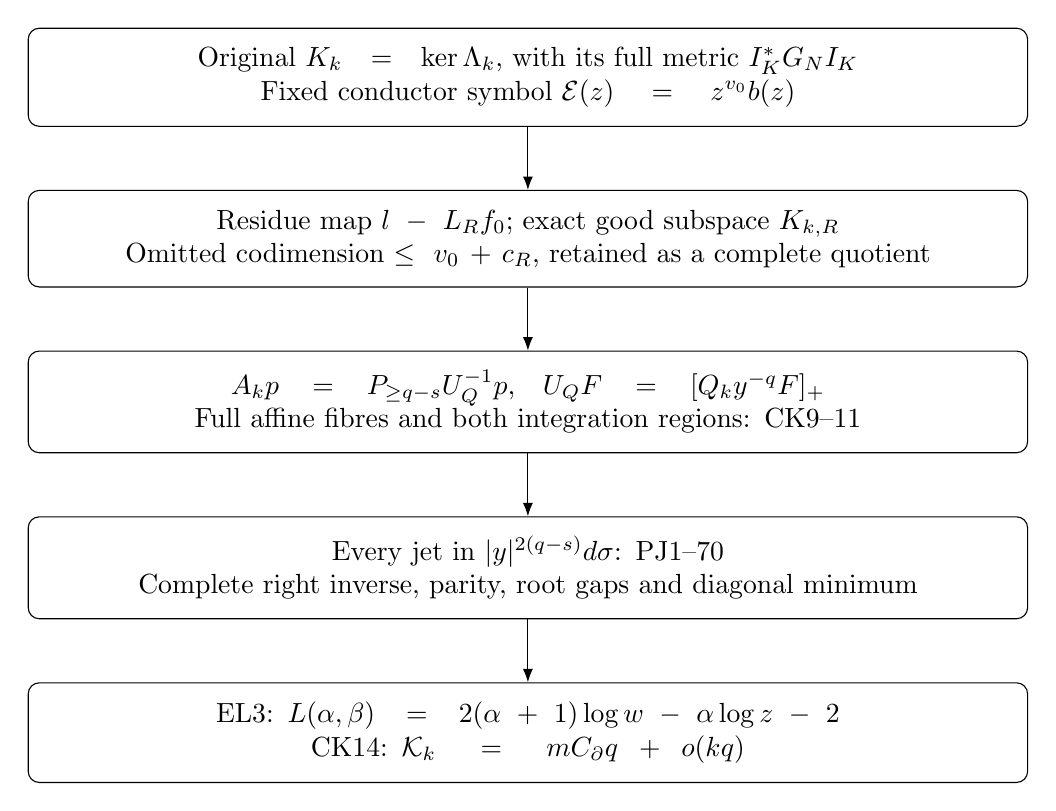
\begin{tikzpicture}[>=Latex,box/.style={draw,rounded corners,align=center,text width=12.2cm,inner sep=7pt}]
\node[box](a){Original $K_k=\ker\Lambda_k$, with its full metric $I_K^*G_NI_K$\\
 Fixed conductor symbol $\mathcal E(z)=z^{v_0}b(z)$};
\node[box,below=8mm of a](b){Residue map $l-L_Rf_0$; exact good subspace $K_{k,R}$\\
 Omitted codimension $\le v_0+c_R$, retained as a complete quotient};
\node[box,below=8mm of b](c){$A_kp=P_{\ge q-s}U_Q^{-1}p$,\quad $U_QF=[Q_ky^{-q}F]_+$\\
 Full affine fibres and both integration regions: CK9--11};
\node[box,below=8mm of c](d){Every jet in $|y|^{2(q-s)}d\sigma$: PJ1--70\\
 Complete right inverse, parity, root gaps and diagonal minimum};
\node[box,below=8mm of d](e){EL3: $L(\alpha,\beta)=2(\alpha+1)\log w-\alpha\log z-2$\\
 CK14: $\mathcal K_k=mC_\partial q+o(kq)$};
\draw[->](a)--(b);\draw[->](b)--(c);\draw[->](c)--(d);\draw[->](d)--(e);
\end{tikzpicture}
\caption{Every arrow is the stated original-coordinate map or complete metric
comparison. CK12 retains the rank-one arithmetic-action defect of $U_Q$.
The complementary quotient costs $O((v_0+c_R)q)$ for each fixed radius;
it is never deleted from the determinant. CK1--14 and PJ1--70 give the
complete proofs. Human Gamma and polynomial sources are credited there.}
\end{figure}\clearpage
\section*{Measured phase and sharp frequency error}
\addcontentsline{toc}{section}{Measured phase and sharp frequency error}
\begin{figure}[H]\centering
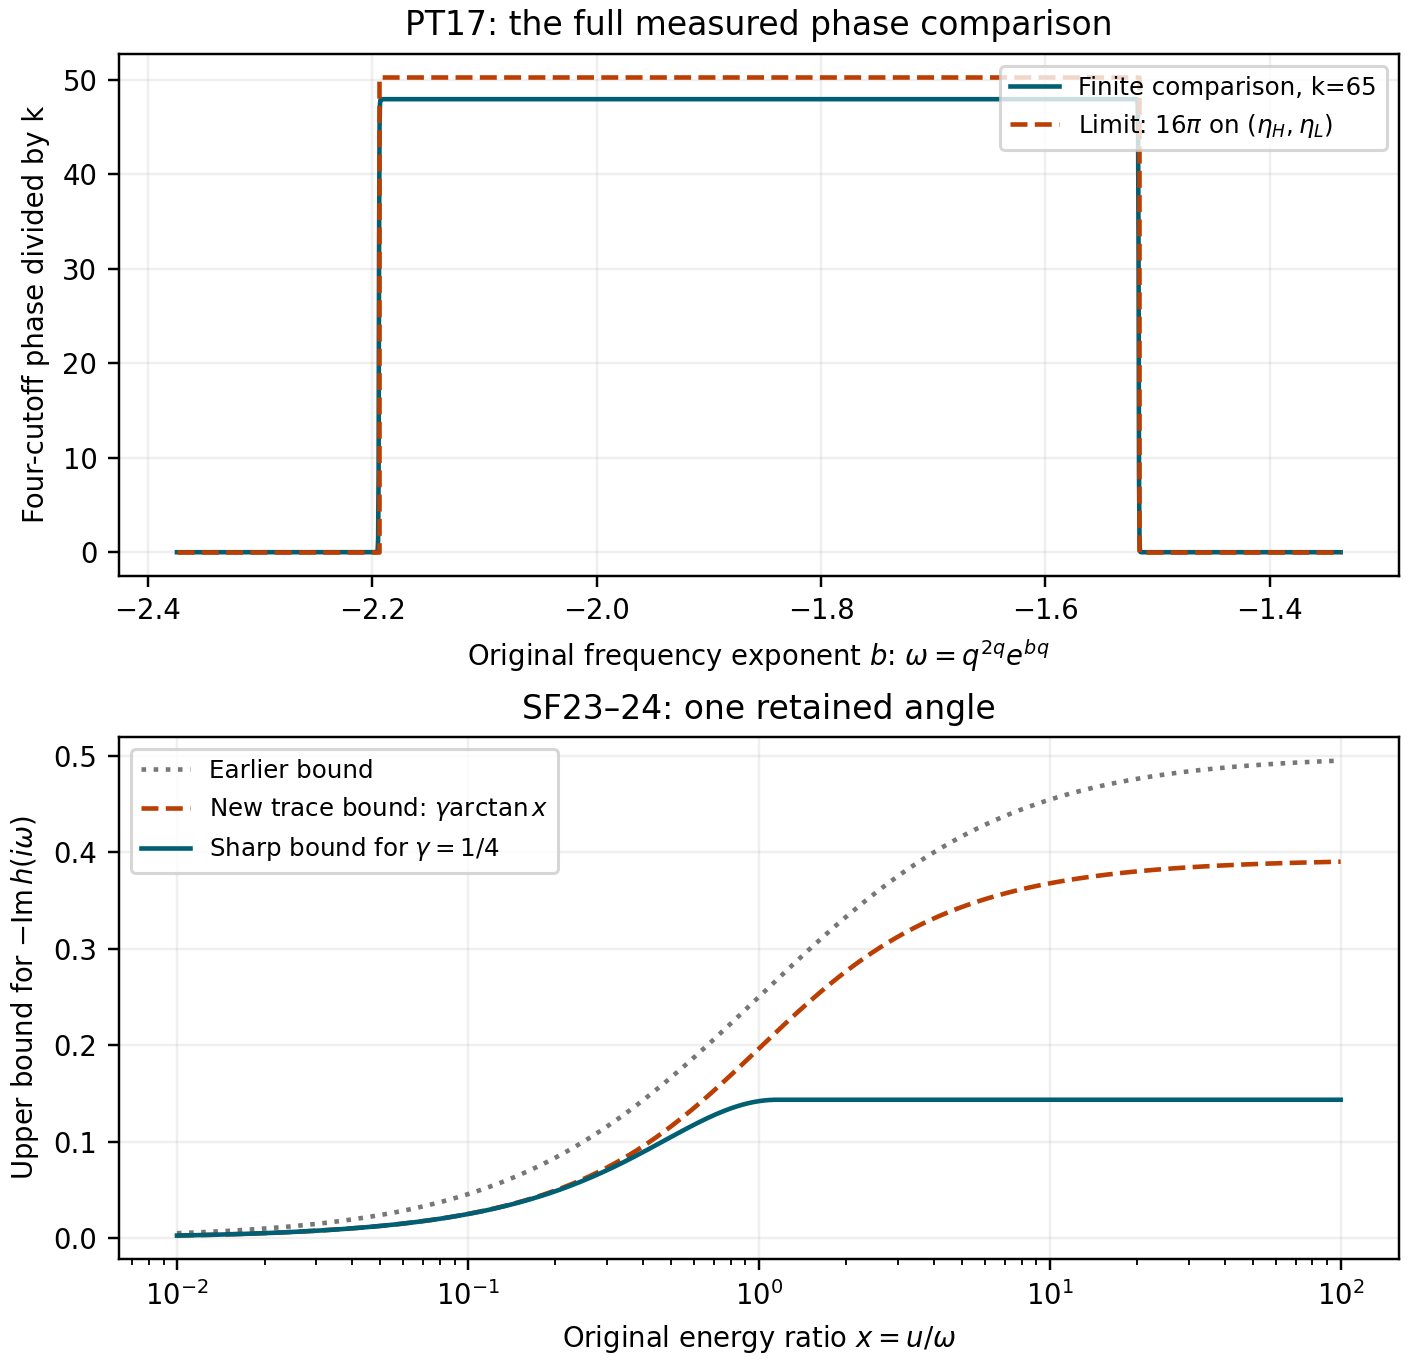
\includegraphics[width=\textwidth]{EXACT_COMPARISONS.png}
\caption{Top: the explicit comparison curve in PT12, at the displayed
finite $k=65$, and the limiting step in PT17. It is not a numerical evaluation
of a native response. PT17 bounds the integral distance of the actual phase
from this curve using the complete original spectra. Bottom: the sharp
one-angle bound SF23--24, with $\gamma=1/4$ and $x=u/\omega$, alongside the
earlier and new trace bounds. SF25--27 construct exact matrices attaining
the sharp curve. The script retains these exact functions; displayed samples
are rounded for plotting.}
\end{figure}
For the entire original phase, PT12 gives
\[
 \int_0^\infty\left|\mathcal R\Theta(\omega)-2\Delta
 \left(\arctan\frac{e^{c_L}}\omega-\arctan\frac{e^{c_H}}\omega\right)\right|
 \frac{d\omega}\omega\le\frac\pi2\mathcal B,
 \qquad\mathcal B=o(kq).
\]
The proof establishes absolute convergence and retains both frequency ends.
The separate complex arithmetic current still uses its original polar insertion.

\clearpage\part{Original kernel and all receiving calculations}
\section{The original kernel value and its receiving calculations}\label{the-original-kernel-value-and-its-receiving-calculations}

This continuation checks all six September22 arrivals together. The full kernel manuscript supplies a fixed-symbol argument. The independent PJ1--69 proof now supplies the complete growing-jet estimate and diagonal asymptotic, and EL1--14 proves the exact identification of its constant. Together they establish the kernel value below. The uniform-return, static-memory, two-response and frequency notes retain their own original maps and receive this value through the equations stated and proved here.

\subsection{CK1. Actual arithmetic objects}\label{ck1.-actual-arithmetic-objects}

Fix the programme's stipulated simple quartet \(0<\delta<1/2\), \(\gamma>2\), its admitted original period and branch, and its arithmetic unit. The result is on that fixed data domain. No zero or period is supplied by the coefficient computation. Keep \[
 k\equiv1\pmod4,\quad k\ge17,\quad q=(k+1)^2,\quad q'=(k-7)^2,
 \quad\Delta=q-q'=16k-48,\quad m=8k-16,
\] \[
 Q_k(y)=\prod_{a,b=0}^k(y-\omega_{ab}),\qquad
 \omega_{ab}=(2b-k)\gamma-i(2a-k)\delta,\qquad S=k/2+iy.
 \tag{CK1}
\] Let \(G_N\) be the full minimum on \(E_k=\mathbb C[y]/(Q_k)\) induced by the original arithmetic source at degree \(N\). Keep its actual observation \(\Lambda_k\) and kernel frame \(I_K\), whose image is \(K_k\) of dimension \(m\). The exact original conductor has the fixed form \[
 \mathcal Tp=\sum_{u,v=0}^8a_{uv}p(y+\sigma_{uv}),\qquad
 \sigma_{uv}=(2v-8)\gamma-i(2u-8)\delta,
\] \[
 \mathcal E(z)=\sum a_{uv}e^{\sigma_{uv}z}=z^{v_0}b(z),\qquad
 b(0)=i^{-v_0}\mu_{v_0}/v_0!\ne0.
 \tag{CK2}
\] The order is denoted \(v_0\) here to keep it distinct from the sum index and the equilibrium endpoint. The original conductor identity is \(p\in K_k\Rightarrow\mathcal Tp=Q_{k-8}\eta\), \(\deg\eta<\Delta-v_0\), with \(\deg p<q\). Only this proved inclusion is used; \(\mathcal T\) does not replace the observation.

The retained complete polynomial comparison to \(d\sigma=|\Gamma(1/4+iy/2)|^2dy/(2\pi)\), of mass \(\sqrt{2\pi}\), is \[
 \ell_k\|P\|_\sigma^2\le\|P\|_{\mu_k}^2\le u_k\|P\|_\sigma^2,
 \qquad\log(u_k/\ell_k)=o(q),\quad\deg P\le2q.
 \tag{CK3}
\] It is the original full-source comparison, before any restriction or minimization. It transfers the four-sign determinant of any fixed rank-\(r\) frame with error at most \(2r\log(u_k/\ell_k)\): each determinant lies between its Gamma determinant plus \(r\log\ell_k\) and plus \(r\log u_k\), and two signs are positive and two negative. Both real integration regions and the source mass remain in CK3.

The target, with its original signs, is \[
 \mathcal K_k=\mathcal R\log\det(I_K^*G_NI_K),\qquad
 \mathcal Rf=f_{q-1}+f_q-f_{2q-1}-f_{2q}.
 \tag{CK4}
\]

\subsection{CK2. Fixed-rank symbol residues and the original quotient}\label{ck2.-fixed-rank-symbol-residues-and-the-original-quotient}

Here are the full finite steps of the kernel manuscript needed to connect CK4 to PJ. In the coefficient norm \(\|p\|_{c,q}=\sum_jq^j|[y^j]p|\), the complete Gamma norms through degree \(2q\) lie between \(e^{-Cq}\|p\|_{c,q}\) and \(e^{Cq}\|p\|_{c,q}\). The upper bound follows from the Gamma moments. For the lower bound the complete Legendre basis on \([1,2]\) bounds coefficients by \(\operatorname{poly}(q)C_0^{2q}\|p(q\cdot)\|_{L^2[1,2]}\); the actual Gamma density on \([q,2q]\) is bounded below by \(cq^{-1/2}e^{-\pi q}\). This bounds the whole-line norm from below without changing it to an interval norm.

The roots of \(q^{-q}Q_k(qx)\) have modulus at most \(\rho_k=k\sqrt{\delta^2+\gamma^2}/q=O(1/k)\). The complete Newton remainder of \(x^j\) has coefficient norm at most \(\sum_{h=0}^j\binom jh2^h=3^j\) for \(j\le2q\): its divided differences are complete homogeneous functions of all actual roots, bounded by \(\binom jh\), and its Newton basis factors have norm at most \(2^h\). Applying this to every representative of a quotient class gives, with one fixed constant, \[
 e^{-C_1q}\|p\|_{c,q}\le\|[p]\|_{G_N^\sigma}\le e^{C_1q}\|p\|_{c,q},
 \qquad\deg p<q,\quad q-1\le N\le2q.
 \tag{CK5}
\] Nesting in \(N\) and full determinant factorization imply that a codimension-\(c\) subspace loses a four-return between zero and \(C_2cq\). Indeed factor the metric on the larger space into its restriction and its complete attained quotient; CK5 bounds every quotient direction, and the same fixed frame is used at all four cutoffs.

Let \(D=\partial_y\) on \(\mathcal P_{q-1}\), so \(\|D\|_{c,q}\le1\). On any fixed circle \(|z|=R>1\) avoiding the zeros of \(b\), let \(M_R=\max|b(z)^{-1}|\) and let \(c_R\) count the interior zeros with multiplicity. The exact resolvent decomposition is \[
 (z-D)^{-1}f=E_{q,z}\lambda_{q,z}(f)-R_zf,
\] \[
 E_{q,z}=\sum_{j<q}(zy)^j/j!,\quad
 \lambda_{q,z}(f)=\sum_{n<q}n![y^n]f\,z^{-n-1},\quad
 R_zf=[e^{zy}\int_0^ye^{-zt}f(t)dt]_{<q}.
 \tag{CK6}
\] For a monomial \(y^n\), the coefficient of \(y^j\) in \(R_zy^n\) is \(n!z^{j-n-1}/j!\) for \(j>n\), and zero otherwise. This verifies CK6 coefficient by coefficient and gives \(\|R_z\|_{c,q}\le qe^{q|z|}\). Define \[
 A_R=\frac1{2\pi i}\oint b(z)^{-1}(z-D)^{-1}dz,\quad
 B_R=\frac1{2\pi i}\oint b(z)^{-1}R_zdz,
\] \[
 L_Rf=\sum_{0<|\zeta|<R}\operatorname{Res}_{z=\zeta}
 [b(z)^{-1}E_{q,z}\lambda_{q,z}(f)].
\] The residue at zero of the first integrand is \(b(D)^{-1}\), since \(D^q=0\) and \(b(0)\ne0\). At each other pole CK6 cancels the \(R_z\) terms, hence \[
 b(D)^{-1}=A_R+B_R-L_R,\quad
 A_R=\sum_{j<q}a_jD^j,\quad |a_j|\le M_RR^{-j},\quad
 \|B_R\|\le RM_Rqe^{Rq},\quad\operatorname{rank}L_R\le c_R.
 \tag{CK7}
\] At an order-\(a\) pole, the range of its residue lies in the \(a\) columns \(\partial_\zeta^jE_{q,\zeta}\), \(0\le j<a\); this proves the rank statement with repeated poles included. The operator \(B_R\) raises degree strictly.

For \(p\in K_k\), put \(f=\mathcal Tp\), and let \(f_0=D^{-v_0}_0f\) be its primitive with all coefficients below \(v_0\) zero. The exact identity \(\mathcal T=D^{v_0}b(D)\) gives \(p=b(D)^{-1}f_0+l(p)\), with \(l(p)\in\mathcal P_{v_0-1}\). Thus the subspace \(K_{k,R}=\{p:l(p)-L_Rf_0=0\}\) has codimension at most \(v_0+c_R\), and \(p=(A_R+B_R)f_0\) there.

The actual lower polynomial in \(f=Q_{k-8}\eta\) has coefficients at depth \(j\) bounded by \(\binom{q'}j\rho_k^j\). Triangular inversion of its leading block bounds \(\|q^{q'}\eta(q\cdot)\|_1\le(1-\rho_k)^{-q'}\|f\|_{c,q}\). Consequently \[
 \|P_{<q'-t}f\|_{c,q}\le(1-\rho_k)^{-q'}2^{q'}\rho_k^t\|f\|_{c,q}.
\] Also \(\|f\|_{c,q}\le(\sum|a_{uv}|e^{|\sigma_{uv}|})\|p\|_{c,q}\) and \(\|f_0\|_{c,q}\le q^{v_0}\|f\|_{c,q}\). For fixed \(\epsilon>0\), these bounds put the coefficients of \(f_0\) below \(q-\epsilon q/2\) at \(\exp[-c_\epsilon q\log k+O(q)]\|p\|_{c,q}\), with \(q-q'=O(k)\) included. In CK7 the high part needs at least \(\epsilon q/2\) derivatives to reach below \(q-\epsilon q\), costing at most \(M_RR^{-\epsilon q/2}/(1-1/R)\). The degree-raising part uses only the small low input. Choosing fixed \(R\) sufficiently large therefore proves, for every fixed \(D_0>0\), \[
 \|P_{<q-\epsilon q}p\|_{c,q}\le e^{-D_0q}\|p\|_{c,q}
 \quad(p\in K_{k,R}),
 \tag{CK8}
\] eventually in \(k\). The radius is fixed after \(\epsilon,D_0\); no uniformity in moving periods is asserted.

\subsection{CK3. Complete source map, every jet, and the exceptional quotient}\label{ck3.-complete-source-map-every-jet-and-the-exceptional-quotient}

Define the actual triangular polynomial map \[
 U_QF=[Q_k(y)y^{-q}F(y)]_+.
 \tag{CK9}
\] Its diagonal is one and it sends \(y^qh\) exactly to \(Q_kh\). Its coefficient norm and inverse norm are \(e^{O(k)}\), bounded by \((1+\rho_k)^q\) and \((1-\rho_k)^{-q}\); coefficients \(j\) places below the diagonal are bounded by \(\binom qj\rho_k^j\) and \(\binom{q+j-1}j\rho_k^j\). For \(s\le q/10\), the complete source comparison is \[
 e^{-C}\|F\|_\sigma^2\le\|U_QF\|_\sigma^2\le e^C\|F\|_\sigma^2,
 \quad F\in y^{q-s}\mathcal P_{N-q+s},\quad q-1\le N\le2q.
 \tag{CK10}
\] Here is the full mechanism. Outside \(|y|<\eta q\), pair all opposite roots in CK1. The logarithm of \(|Q_k/y^q|^2\) is bounded by a constant times \(qk^2/|y|^2=O(1)\). In the coordinate \(x=y/q\), write \(F(qx)=x^{q-s}b(x)\). The negative Laurent part of \(x^{-s}q^{-q}Q_k(qx)b(x)\) has coefficient sum at most \(2^q\rho_k^{q-s}\|b\|_1\). Its exterior norm is \(\exp[-(1-s/q)q\log k+O(q)]\|b\|_1\), negligible by CK5's pre-minimum coefficient bound.

For the two inner integrals, Cauchy's polynomial-part formula on \(|z|=2\eta\) gives \(|U_QF(qx)|\le2(2\eta+\rho_k)^q(2\eta)^{-s}\sup_{|z|=2\eta}|b(z)|\) for \(|x|\le\eta\). The Legendre coefficient estimate gives \(\sup_{|z|\le2\eta}|b(z)|\le\operatorname{poly}(q)10^{\deg b}\|b\|_{L^2[1,2]}\). The contribution of \([q,2q]\) to \(\|F\|_\sigma^2\) is at least \(c\sqrt q e^{-\pi q}\|b\|_{L^2[1,2]}^2\). The logarithm of the inner-to-total ratio is bounded by \(q[\pi+2(1+1/10)\log10+2(1-1/10)\log(2\eta)+o(1)]\), negative by a fixed margin for \(\eta=2^{-32}\). The same estimate directly bounds the inner integral of \(F\). Combining these two small integrals with the exterior estimates proves CK10. No Laurent expression is integrated through zero.

The complete affine fibres correspond exactly: \[
 f+y^q\mathcal P_{N-q}\ \xrightarrow{\ U_Q\ }\ U_Qf+Q_k\mathcal P_{N-q},
 \qquad f\in y^{q-s}\mathcal P_{s-1}.
 \tag{CK11}
\] Thus CK10 passes to complete minima. Taking CK8 first with half as wide a band, and using the inverse coefficient tails in CK9, gives the cutoff-independent injective map \(A_kp=P_{\ge q-s}U_Q^{-1}p\) from \(K_{k,R}\) into \(y^{q-s}\mathcal P_{s-1}\), with relative \(e^{-cq}\) error in each original quotient norm. This follows because its coefficient error is \(e^{-D_0q/2}\|p\|_{c,q}\) and CK5 bounds both original norms, with \(D_0\) chosen larger than their fixed exponents. Injectivity follows from the same strict relative bound.

This map retains the exact arithmetic-action defect. If \(Q_k=\sum_{j=0}^qc_jy^j\), then, on representatives of degree below \(q\), \[
 M U_Q-U_QM_0=-[1](c_{q-1},c_{q-2},\ldots,c_0),
 \tag{CK12}
\] where \(M\) is multiplication modulo \(Q_k\) and \(M_0\) multiplication modulo \(y^q\). Multiplying each polynomial part proves this identity on every basis monomial. CK11 is a metric comparison, with this rank-one action defect retained.

The independent PJ1--69 and EL1--14 proofs now give, for every coefficient vector in that power band and both original low/high pairs, \[
 \log\frac{\|f\|_{G_l^{\rm pow}}^2}{\|f\|_{G_u^{\rm pow}}^2}
 =\frac{C_\partial q}{2}
 +O\{s\log(Cq/s)+s+\log q\}+o(q).
 \tag{CK13}
\] The proof of every direction is the full jet right inverse PJ34--38, the complete low Gram PJ19--25, and fixed-degree power transport PJ39--45. The scalar diagonal sequence is proved by the monic minimum and zero-law arguments PJ52--69, including both regions and the exact Gamma mass; EL12 identifies its coefficient. These complete proofs accompany this note. In particular no derivative is taken of an unquantified moving-degree error.

Apply CK13 to the image of \(A_k\) and then CK10--11. It holds for every vector of \(K_{k,R}\), so generalized min--max bounds every low/high eigenvalue on that restricted subspace. If its dimension is \(m-c\), its two-pair determinant return differs from \((m-c)C_\partial q\) by at most \((m-c)q[O(\epsilon\log(C/\epsilon))+o(1)]\), with \(s=\lfloor\epsilon q\rfloor\). The complete exceptional quotient in CK5 costs at most \(C_2cq\), where \(c\le v_0+c_R\) is fixed for fixed \(\epsilon\). Divide by \(mq\), let \(k\to\infty\), and then let \(\epsilon\downarrow0\). Since \(m\to\infty\), the exceptional term tends to zero. Finally CK3 returns to the actual arithmetic metric. This proves \[
 \boxed{\mathcal K_k=(8k-16)C_\partial q+o(kq).}
 \tag{CK14}
\] The same proof on any cutoff-independent subspace of the original conductor kernel, of rank \(r_k\to\infty\) and \(r_k\le\Delta\), gives \(r_kC_\partial q+o(r_kq)\). The codimension removed is at most the same fixed \(v_0+c_R\); division by \(r_k\), followed by the same ordered limits, justifies even slower-growing ranks.

\subsection{CK4. Relative spectra and the original measured determinant}\label{ck4.-relative-spectra-and-the-original-measured-determinant}

The relative kernel eigenvalues are bounded by \(e^{O(q)}\) in both directions, by CK5 and CK3. At most twice the discarded codimension lies outside the interval in CK13, by generalized min--max on the fixed subspace. Therefore, for each original pair \((l,u)\), \[
 \Omega_{l,u}:=\sum_{j=1}^m\left|\log\lambda_j(H_{K,u}^{-1/2}H_{K,l}H_{K,u}^{-1/2})
 -C_\partial q/2\right|=o(kq).
 \tag{CK15}
\] This is more information than the signed determinant alone. It is the precise input required by the earlier uniform-return manuscript.

To spell out its noncommuting transport, let \(P,Q,F>0\) be metrics and an energy form on one fixed coefficient space. Put \(R=P^{1/2}\max(I,P^{-1/2}QP^{-1/2})P^{1/2}\). Then \(R\succeq P,Q\), and generalized min--max bounds each decreasing \(\lambda_j(F,R)\) below those for \(P,Q\). Pairing ordered logarithms through this common lower list proves \[
 \sum_j|\log\lambda_j(F,P)-\log\lambda_j(F,Q)|
 \le\log\frac{\det R}{\det P}+\log\frac{\det R}{\det Q}
 =\sum_j|\log\lambda_j(P^{-1/2}QP^{-1/2})|.
 \tag{CK16}
\] The equality follows by splitting the eigenvalues of \(P^{-1/2}QP^{-1/2}\) above and below one. No common eigenvectors of \(P,Q,F\) are assumed.

For the original word \(T=D_k(M)\), retain the full positive-energy band \(e^{c_N-e_k}P_{(\ker T)^{\perp_{G_N}}}\preceq_{G_N}T^{\dagger_{G_N}}T\preceq_{G_N}e^{c_N+e_k}P_{(\ker T)^{\perp_{G_N}}}\), with \(e_k=o(q)\), \[
 c_L=2q\log q+\eta_Lq,\quad c_H=c_L-C_\partial q/2,
 \quad\eta_L=2\log(4/\pi)-2.
 \tag{CK17}
\] These are the original measured-word and uniform-return inputs. Their complete boundary quotient in a common fixed value frame has logarithmic width \(o(q)\). Thus for \(F_N=(TI_K)^*G_N(TI_K)\), its scaled low/high comparison has width \(o(q)\) about \(e^{C_\partial q/2}\). Apply CK16 first with the same energy and kernel metrics, and then min--max to the actual energy comparison. Equation CK15 gives \(D_i=\sum_j|\log\alpha_{j,N_i}-\log\alpha_{j,N_{i+2}}|=o(kq)\), in precisely PT10's notation.

The full observed determinant PT4 now yields, because \(a\mapsto\log(1+e^a/z)\) is 1-Lipschitz for every \(z>0\), \[
 \boxed{\sup_{z>0}\left|\mathcal R\log\det\mathscr Y_N(z)
 +2\Delta\log\frac{z+e^{c_L}}{z+e^{c_H}}\right|
 \le D_0+D_1+4\Delta e_k=o(kq).}
 \tag{CK18}
\] In particular the original, unextended observation has root-scale and all lower positive-scale return \(-\Delta C_\partial q+o(kq)\). The formula is uniform for positive \(z\); it does not take the logarithm of an individual singular response at zero. The earlier depth-eight bound remains valid on its extra corner-period guards and now connects to the same original leading plateau via its exact attained compression.

\subsection{CK5. Earlier receivers updated at their actual scope}\label{ck5.-earlier-receivers-updated-at-their-actual-scope}

The following replacements use their complete earlier equations, not their ranks in isolation.

\begin{enumerate}
\def\labelenumi{\arabic{enumi}.}
\tightlist
\item
  \textbf{Invariant-row covariance.} Its retained exact receiving equation is \(\mathcal K_k=(\Delta-v_0)C_\partial q+\mathcal R\log\det S_N+o(kq)\). Subtract CK14 to obtain \(\mathcal R\log\det S_N=-(\Delta-v_0-m)C_\partial q+o(kq)\). A fixed-rank difference remains \(O(q)\); it is not an evaluated order-\(q\) coefficient.
\item
  \textbf{Selected arithmetic layers.} AP's actual interval is \(0\le\mathcal K_k-X_s\le2t_s\mathfrak E_k\), with \(\mathfrak E_k=O(q)\). Hence any fixed layer with \(t_s=O(1)\), including its proved depth-eight domain, has \(X_s=mC_\partial q+o(kq)\). For growing remaining layers the complete quotient theorem following CK14 gives their own rank coefficient. No arbitrary layer distribution is inferred from a total alone.
\item
  \textbf{Two measured responses.} With the original \(Q_N\) metric, the positive secant is \(Z_N=12(2I+\mathscr Y_N(2\sigma/3))^{-1}-4(I+\mathscr Y_N(\sigma/2))^{-1}-2I\). Its proof gives \(-2W_k\le\mathcal K_k+\mathcal R\log e_{m-h_k}(Z_N)\le2m\omega_k+2W_k\), where \(W_k=O(q\log q)\), \(h_k=O(1)\), \(\omega_k=o(q)\). Thus its actual positive characteristic coefficient has return \(-mC_\partial q+o(kq)\). This is a leading signed return; individual coefficients and numerical sample precision are retained separately in S10--13.
\item
  \textbf{Static and dynamic memory.} The static proof's exact matrices are \(S=C^*A^{-1}C\), \(E_0=B_0-S\), and \(\Sigma(z)=C^*(z+A)^{-1}C\). They are connected by \(S-\Sigma(z)=zC^*A^{-1}(z+A)^{-1}C\). Its static root returns are \(mC_\partial q\), \(\Delta C_\partial q\), and \((\Delta-m)C_\partial q\), each with its proved \(o(kq)\) remainder. Its dynamic receiver is \(\mathcal RD_N(z)=mC_\partial q-\mathcal K_k+o(kq)\), so CK14 makes this \(o(kq)\) on the stated root domain. It does not make any individual dynamic determinant zero.
\item
  \textbf{Frequency recovery.} PT12--22 now receive \(\mathcal B=D_0+D_1+\sum_NE_N=o(kq)\), since \(\sum_NE_N\le4\Delta e_k\). They prove the entire measured phase transition in integral norm, with finite error, and the controlled root-scale phase-area correction. The new independent SF1--36 sharp angle bounds further strengthen the frequency error. These equations supersede the newest archive's isolated statement that its leading determinant coefficient is unevaluated.
\item
  \textbf{Short ambient and hidden quotients.} PEN17--20's two operations remain connected by their actual terminal metric, of rank at most128. Its two-sided \(O(q)\) correction is retained. Consequently both full proved receivers have the same \(kq\) coefficient where their old intervals transfer \(\mathcal K_k\), while their finite signs and order-\(q\) terms remain distinct.
\end{enumerate}

The projected complex arithmetic currents still require their original phase-bearing insertions. Equal positive energies can correspond to different polar actions. The determinant and measured-resolvent phase results above therefore do not assign those current signs or remove the retained positive canonical action. This scope is part of the theorem, not a conclusion that the programme has ended.

\textbf{Two-response proof correction.} In the explanatory sentence following the incoming S2, the filtered secant needs its outer factor two. With \(Y^{(\sigma)}(x)=(xI+Y(\sigma x/(1+x)))/(1+x)\), the exact formula is \[
 Z=2\{2Y^{(\sigma)}(2)^{-1}-Y^{(\sigma)}(1)^{-1}-I\}
 =2C^*(I+A)^{-1}(2I+A)^{-1}C.
 \tag{CK19}
\] The blocks in the last expression are those of the filtered energy. The complete filtered Schur identity gives \(xY^{(\sigma)}(x)^{-1}=xI+B_0-C^*(xI+A)^{-1}C\); subtract its values at two and one to prove CK19. Substitution of the displayed response map then gives exactly the coefficients12,4,2 in the original secant. Thus the source's displayed S1 and S2 are unchanged, while their connecting sentence is corrected. The independent original-metric checker includes a negative control rejecting omission of this factor.

\subsection{Provenance and proof sources}\label{provenance-and-proof-sources}

This proof uses the user-supplied \emph{The original kernel coefficient}, full14-page manuscript, Sections1--7; the full earlier uniform-return and static-memory proofs; the two-response proof S1--13; and frequency FD10--24. All six arrivals and every supporting file are individually recorded in \texttt{INTAKE\_REVIEW.json}. The complete independent PJ, EL, PT and SF proofs accompany this continuation. Original source PDFs are preserved; the mathematical transcription and additional derivations here are identified as such.

The retained human Gamma and polynomial sources are cited in PJ's source ledger. The elliptic source and its actual reading/fetch status are in EL. Existing full-programme sources include \href{https://github.com/KokunoYumeto/zeta-function-research-reader/blob/9104d852c6bc5b79e6fc4588c403128a40b7fda3/workbenches/splitzero-tandem/continuations/20260922-arithmetic-probe-mass/PROBE_PROOFS.md}{AP1--30}, \href{https://github.com/KokunoYumeto/zeta-function-research-reader/blob/9104d852c6bc5b79e6fc4588c403128a40b7fda3/workbenches/splitzero-tandem/continuations/20260922-arithmetic-probe-mass/MASS_PROOFS.md}{KM1--45}, and \href{https://github.com/KokunoYumeto/zeta-function-research-reader/blob/9104d852c6bc5b79e6fc4588c403128a40b7fda3/workbenches/splitzero-tandem/continuations/20260922-arithmetic-probe-mass/PENCIL_PROOFS.md}{PEN1--27}. Those frozen proofs are preserved. The new claims above strengthen their receiving values; they do not rewrite their source history.

\clearpage\part{The complete Gamma-power minimum}
\section{The complete Gamma-power jet minimum}\label{the-complete-gamma-power-jet-minimum}

Independent derivation, 22 September 2026. This proof addresses §§6.1--6.3 of the supplied \emph{The original kernel coefficient}. It proves the complete finite comparison in the original measure and reduces its scalar part to an explicitly displayed diagonal remainder. It assigns no new coefficient to the original arithmetic kernel.

\subsection{PJ1. Original measure, mass, cutoffs and coefficient maps}\label{pj1.-original-measure-mass-cutoffs-and-coefficient-maps}

Retain

\[
d\sigma(y)=w(y)\,dy,\qquad
w(y)=\frac{|\Gamma(1/4+iy/2)|^2}{2\pi},\qquad
d\nu_n(y)=|y|^{2n}d\sigma(y),\qquad
d_n=\int_{\mathbb R}d\nu_n.
\tag{PJ1}
\]

Its complete mass is \(d_0=\sqrt{2\pi}\). To verify the scalar, put \(g_a(u)=e^{au-e^u}\), \(a>0\). The substitution \(x=e^u\) gives \(\int g_a(u)e^{itu}\,du=\Gamma(a+it)\). Plancherel and the substitution \(x=e^u\) give

\[
\int_{\mathbb R}|\Gamma(a+it)|^2\frac{dt}{2\pi}
=\int_{\mathbb R}e^{2au-2e^u}\,du=2^{-2a}\Gamma(2a).
\]

The original variable is \(y=2t\), so its measure contributes twice this integral. At \(a=1/4\) this is \(2^{1/2}\Gamma(1/2)=\sqrt{2\pi}\). None of the measures in (PJ1) is divided by its mass.

Let \(\mathcal P_m=\{P\in\mathbb C[y]:\deg P\le m\}\). For integers \(q\ge40\) and \(1\le s\le q/10\), set \(n=q-s\), and define the surjective linear map

\[
J_{q,s}:\mathcal P_m\longrightarrow\mathbb C^s,
\qquad (J_{q,s}P)_j=q^j[y^j]P(y),\quad0\le j<s,
\qquad m\ge s-1.
\tag{PJ2}
\]

The positive Hermitian minimum metric \(H_{n,m}^{(q,s)}\) is specified by

\[
a^*H_{n,m}^{(q,s)}a
=\min\{\|P\|_{\nu_n}^2:P\in\mathcal P_m,\ J_{q,s}P=a\}.
\tag{PJ3}
\]

Existence and uniqueness follow from orthogonal projection onto the finite-dimensional affine fibre; positivity follows because its homogeneous coefficient map is surjective. All coefficients may be complex. The four original power-quotient cutoffs correspond exactly to

\[
\begin{array}{c|cccc}
N&q-1&q&2q-1&2q\\ \hline
m=N-(q-s)&s-1&s&q+s-1&q+s.
\end{array}
\tag{PJ4}
\]

Indeed \(F(y)=y^{q-s}P(y)\) has norm \(\|P\|_{\nu_n}\), and the relation \(F\bmod y^q\) prescribes exactly (PJ2). Multiplication by \(y^{q-s}\) is a bijection between these polynomial fibres and the original power-quotient fibres. This proves the norm correspondence, including the source degree, rather than merely identifying two coefficient lists.

\subsection{PJ2. The full Laguerre derivative matrix and inverse moments}\label{pj2.-the-full-laguerre-derivative-matrix-and-inverse-moments}

The auxiliary comparison measure is

\[
d\lambda_n(y)=|y|^{\alpha}e^{-\theta|y|}\,dy,
\qquad \alpha=2n-\tfrac12,\quad\theta=\pi/2.
\tag{PJ5}
\]

It is a separate explicitly defined measure used to bound (PJ1). On the positive half-line write \(\|\cdot\|_{\alpha,\theta}\) for its norm. The original DLMF equations \href{https://dlmf.nist.gov/18.9.E23}{18.9.23} and \href{https://dlmf.nist.gov/18.9.E13}{18.9.13}, read in their original equation TeX, imply

\[
\frac{d}{dz}L_j^{(\alpha)}(z)
=-L_{j-1}^{(\alpha+1)}(z)
=-\sum_{i=0}^{j-1}L_i^{(\alpha)}(z).
\tag{PJ6}
\]

For completeness, the finite expression \href{https://dlmf.nist.gov/18.5.E12}{DLMF 18.5.12} gives the Rodrigues identity by the product rule. Integrating that identity by parts \(j\) times against \(z^i\), with \(i<j\), proves orthogonality; the boundary terms vanish because \(\alpha>-1\) and the differentiated factor is \(z^{j+\alpha}e^{-z}\). The same calculation against the leading term \((-1)^jz^j/j!\) proves

\[
\int_0^\infty L_i^{(\alpha)}(\theta y)L_j^{(\alpha)}(\theta y)
y^\alpha e^{-\theta y}\,dy
=\mathbf1_{i=j}\,h_j,
\quad h_j=\theta^{-\alpha-1}\frac{\Gamma(j+\alpha+1)}{j!}.
\tag{PJ7}
\]

In the orthonormal basis \(L_j^{(\alpha)}(\theta y)/\sqrt{h_j}\), the derivative matrix therefore has, for \(i<j\), the exact entry

\[
D_{ij}=-\theta\sqrt{\frac{j!\Gamma(i+\alpha+1)}{i!\Gamma(j+\alpha+1)}}
=-\theta\prod_{r=i+1}^j\sqrt{\frac r{r+\alpha}}.
\tag{PJ8}
\]

For \(n\ge2\) and degree \(d\le2n+2\), put \(\rho=(2n+2)/(4n+3/2)\). Then \(\rho\le12/19<16/25\). Hence each absolute row sum and each absolute column sum is at most

\[
\theta\sum_{j\ge1}\rho^{j/2}
=\theta\frac{\sqrt\rho}{1-\sqrt\rho}<4\theta.
\]

The inequality \(\|D\|_2^2\le\|D\|_1\|D\|_\infty\), proved by applying weighted Cauchy--Schwarz in each row and summing, now gives the full, degree-uniform estimate

\[
\|P'\|_{\alpha,\theta}\le4\theta\|P\|_{\alpha,\theta},
\qquad P\in\mathcal P_{2n+2},\ n\ge2.
\tag{PJ9}
\]

The same estimate applies to \(P(-y)\) on the positive half-line, including its derivative sign.

Put \(N=\|P\|_{\alpha,\theta}^2>0\), \(B_1=N^{-1}\int_0^\infty|P|^2y^{\alpha-1}e^{-\theta y}dy\), and \(B_2=N^{-1}\int_0^\infty|P|^2y^{\alpha-2}e^{-\theta y}dy\). Integrating the derivatives of \(|P|^2y^\alpha e^{-\theta y}\) and \(|P|^2y^{\alpha-1}e^{-\theta y}\) gives, with \(L=4\theta\),

\[
\alpha B_1\le\theta+2L,
\qquad
(\alpha-1)B_2\le\theta B_1+2L\sqrt{B_2}.
\tag{PJ10}
\]

The boundary terms vanish at infinity and at zero, since \(\alpha>1\). For \(z=\sqrt{B_2}\), solving the resulting quadratic and using \(\sqrt{L^2+(1-1/\alpha)\theta(\theta+2L)}\le L+\theta\) yields

\[
\left\|\frac P y\right\|_{\alpha,\theta}
\le\frac{2L+\theta}{\alpha-1}\|P\|_{\alpha,\theta}
\le\frac{8\theta}{n}\|P\|_{\alpha,\theta}.
\tag{PJ11}
\]

Summing the squared inequalities for \(P(y)\) and \(P(-y)\) gives the same estimate in \(\lambda_n\). The rational expression \(P/y\) is integrated with its actual weight; no assertion that it is a polynomial is needed.

The Laguerre recurrence can also be checked coefficient by coefficient in the same finite expression:

\[
zL_j^{(\alpha)}(z)=-(j+1)L_{j+1}^{(\alpha)}(z)
+(2j+\alpha+1)L_j^{(\alpha)}(z)-(j+\alpha)L_{j-1}^{(\alpha)}(z).
\]

In the orthonormal basis its off-diagonal magnitudes are \(\sqrt{(j+1)(j+\alpha+1)}/\theta\). The row and column sums of the multiplication matrix, including its last raising row, are at most \(20n/\theta\) through source degree \(2n+1\), for \(n\ge2\). For example its entries are bounded by the diagonal \((6n+7/2)/\theta\) and two copies of \(\sqrt{(2n+2)(4n+3/2)}/\theta\); their sum is less than \(20n/\theta\). Thus

\[
\|yP\|_{\lambda_n}\le\frac{20n}{\theta}\|P\|_{\lambda_n},
\qquad\deg P\le2n+1.
\tag{PJ12}
\]

\subsection{PJ3. The near-zero Gamma comparison and full multiplication bounds}\label{pj3.-the-near-zero-gamma-comparison-and-full-multiplication-bounds}

The original Gamma asymptotic \href{https://dlmf.nist.gov/5.11.E9}{DLMF 5.11.9}, read as equation TeX, gives

\[
g(x):=x^{1/2}e^{\theta x}w(x)\longrightarrow\sqrt2
\quad(x\to+\infty).
\]

The positive function \(g\) is continuous on \((0,\infty)\), extends continuously with \(g(0)=0\), and has no zero for \(x>0\). Consequently

\[
A:=\inf_{x\ge1}g(x)>0,\qquad
B:=\sup_{x\ge0}g(x)<\infty.
\tag{PJ13}
\]

In particular a global \emph{pointwise} lower comparison to (PJ5) would be false at zero. The following argument supplies the required whole-polynomial lower comparison. By (PJ11), for \(\deg P\le2n+2\),

\[
\int_{|y|<1}|P|^2d\lambda_n
\le\int\frac{|P|^2}{|y|^2}d\lambda_n
\le\frac{64\theta^2}{n^2}\|P\|_{\lambda_n}^2.
\]

Our range has \(n\ge36>16\theta\), so the last factor is at most \(1/4\). Applying the upper pointwise comparison everywhere and the lower comparison on \(|y|\ge1\) proves

\[
\frac A2\|P\|_{\lambda_n}^2
\le\|P\|_{\nu_n}^2\le B\|P\|_{\lambda_n}^2,
\qquad\deg P\le2n+2.
\tag{PJ14}
\]

The constant polynomial gives the same two bounds between the complete masses \(d_n\) and \(\lambda_n(\mathbb R)\). Define \(\kappa=\sqrt{2B/A}\). The upper pointwise comparison also applies directly to the integrable function \(P/y\). Combining it with (PJ11), (PJ12), and the lower bound in (PJ14), yields

\[
\|P/y\|_{\nu_n}\le\frac{8\theta\kappa}{n}\|P\|_{\nu_n},
\qquad
\|yP\|_{\nu_n}\le\frac{20\kappa n}{\theta}\|P\|_{\nu_n}.
\tag{PJ15}
\]

Cauchy--Schwarz applied to \(P/y\) and \(yP\) supplies the missing lower raising bound. Thus there are fixed \(0<c\le1\le C\) such that

\[
cn\|P\|_{\nu_n}\le\|yP\|_{\nu_n}\le Cn\|P\|_{\nu_n},
\qquad\deg P\le2n+1,
\tag{PJ16}
\]

with the last raising degree included. One may take the smaller of \(1,(8\theta\kappa)^{-1}\) for \(c\) and the larger of \(1,20\kappa/\theta\) for \(C\). These are fixed constants attached to the literal Gamma density, not to \(q,s\) or a coefficient direction.

\subsection{PJ4. Root gaps, including the odd zero}\label{pj4.-root-gaps-including-the-odd-zero}

Let \(U_j^{[n]}\) be the monic degree-\(j\) polynomial orthogonal for \(\nu_n\), and \(h_j^{[n]}=\|U_j^{[n]}\|_{\nu_n}^2\). The density is positive away from one point, so its polynomial Gram matrices are positive definite. Uniqueness and the even density give \(U_j^{[n]}(-y)=(-1)^jU_j^{[n]}(y)\).

Under the actual map \(x=y^2\), the pushforward measure is

\[
d\rho_n(x)=\frac{x^{n-1/2}}{2\pi}
|\Gamma(1/4+i\sqrt{x}/2)|^2\,dx,\qquad x>0.
\tag{PJ17}
\]

Indeed the two half-lines each contribute \(dy=dx/(2\sqrt{x})\); both are retained. Thus \(U_{2m}^{[n]}(y)=R_m(y^2)\), where \(R_m\) is monic orthogonal for \(\rho_n\), and \(U_{2m+1}^{[n]}(y)=yS_m(y^2)\), where \(S_m\) is monic orthogonal for \(x\,d\rho_n\). These assertions follow by substituting every even test monomial in the original orthogonality identities; odd test monomials vanish by parity.

For any positive measure with all moments and positive polynomial Gram matrices, the zeros of its monic degree-\(m\) orthogonal polynomial are the eigenvalues of multiplication by \(x\) compressed to \(\mathcal P_{m-1}\). To verify this statement, use the orthonormal polynomial basis: multiplication is tridiagonal because \(\langle xp_j,p_i\rangle=\langle p_j,xp_i\rangle=0\) for \(i<j-1\). Its off-diagonal coefficients are positive ratios of leading coefficients. Expansion of the compressed characteristic determinant along its last row gives the identical monic three-term recurrence and the initial determinants \(1\) and \(x-b_0\). Hence the determinants are precisely the monic orthogonal polynomials. A symmetric tridiagonal matrix with all off-diagonal entries nonzero has simple eigenvalues: an eigenvector is determined by its first coordinate, and a zero first coordinate forces every coordinate to vanish. The recurrence, evaluated at consecutive simple zeros, gives strict interlacing by alternating signs and the leading signs at infinity.

For the \(\rho_n\) compression its Rayleigh quotient at a polynomial \(R\) is exactly

\[
\frac{\int x|R(x)|^2d\rho_n}{\int|R(x)|^2d\rho_n}
=\frac{\|yR(y^2)\|_{\nu_n}^2}{\|R(y^2)\|_{\nu_n}^2}.
\]

For the \(x\rho_n\) compression the same quotient is \(\|y^2R(y^2)\|_{\nu_n}^2/\|yR(y^2)\|_{\nu_n}^2\). Every polynomial on the right is within the degree range of (PJ16) for all uses below. Therefore all the compressed eigenvalues lie in \([c^2n^2,C^2n^2]\). Consequently every nonzero root of each used \(U_j^{[n]}\) lies in

\[
[-Cn,-cn]\ \cup\ [cn,Cn].
\tag{PJ18}
\]

An odd polynomial has exactly its one additional simple root at zero. It is never included in a product that is divided by a nonzero root. In particular (PJ18) applies to all degrees at most \(2n+2\), since the Rayleigh source polynomial has degree at most \(j-2\).

\subsection{PJ5. Low degree: the full coefficient metric}\label{pj5.-low-degree-the-full-coefficient-metric}

For \(0\le j\le s\), use polynomials monic in the actual scaled coefficient variable \(x=y/q\):

\[
\ell_j(x)=\frac{(-1)^j j!}{(\theta q)^j}L_j^{(\alpha)}(\theta qx).
\]

By (PJ7), their squared norms for the positive half-line, divided only here to express the ratio to that half-line's complete mass, are

\[
\frac{\|\ell_j(y/q)\|_{\alpha,\theta}^2}
{\Gamma(\alpha+1)\theta^{-\alpha-1}}
=\frac{j!(\alpha+1)_j}{(\theta q)^{2j}}.
\tag{PJ19}
\]

Since \(9q/10\le n\le q\) and \(j\le s\le q/10\), every factor \((\alpha+r)/(\theta^2q)\), \(1\le r\le j\), is between two fixed positive constants. The elementary bounds \((j/e)^j\le j!\le j^j\) then give, uniformly for \(0\le j\le s\),

\[
e^{-s\log(C_1q/s)-C_1s}
\le\frac{j!(\alpha+1)_j}{(\theta q)^{2j}}\le e^{C_1s}.
\tag{PJ20}
\]

At \(j=0\) the ratio is exactly one. For the lower bound at \(1\le j\le s\), use monotonicity of \(u\mapsto u\log(C_1q/u)\) on this interval, increasing \(C_1\) if necessary.

The finite Laguerre expansion gives

\[
[x^i]\ell_j(x)
=(-1)^{j-i}\binom ji\frac{(\alpha+i+1)_{j-i}}{(\theta q)^{j-i}}.
\tag{PJ21}
\]

The inverse triangular transformation has exactly the same coefficients without the sign:

\[
x^j=\sum_{i=0}^j\binom ji
\frac{(\alpha+i+1)_{j-i}}{(\theta q)^{j-i}}\ell_i(x).
\tag{PJ22}
\]

To verify (PJ22), substitute (PJ21). In the coefficient at \(x^r\), the product of the two rising factorials is always \((\alpha+r+1)_{j-r}\), and the remaining sum is \(\binom jr\sum_{i=r}^j(-1)^{i-r}\binom{j-r}{i-r}\), equal to zero for \(r<j\) and one for \(r=j\). All entries in both transformations are at most \(\binom jiC_2^{j-i}\) in absolute value. Their Euclidean operator norms are at most \((s+1)(1+C_2)^s\). Combining (PJ19)--(PJ22) therefore controls the whole coefficient Gram, rather than individual monomial norms.

On the negative half-line the change from \(P(y)\) to \(P(-y)\) is the diagonal unitary coefficient map \(a_j\mapsto(-1)^ja_j\), so the same lower and upper bounds hold there. Summing both halves and using (PJ14), including its constant-polynomial mass comparison, proves the following with a fixed enlarged constant \(C_3\): put

\[
E_0(q,s)=C_3\{s\log(C_3q/s)+s+\log(q+2)\}.
\tag{PJ23}
\]

For every \(P(y)=\sum_{j=0}^{s}b_j(y/q)^j\),

\[
d_ne^{-E_0}\|b\|_2^2\le\|P\|_{\nu_n}^2
\le d_ne^{E_0}\|b\|_2^2.
\tag{PJ24}
\]

At degree \(s-1\), (PJ24) is the desired metric directly. At degree \(s\), every complete fibre has coefficient vector \((a,b_s)\). The lower bound survives because \(\|(a,b_s)\|_2\ge\|a\|_2\); the upper bound follows by selecting \(b_s=0\). Hence the \emph{attained} low metrics obey

\[
d_ne^{-E_0}I\preceq H_{n,s-1}^{(q,s)},\ H_{n,s}^{(q,s)}
\preceq d_ne^{E_0}I.
\tag{PJ25}
\]

\subsection{PJ6. The complete high covariance: upper bound}\label{pj6.-the-complete-high-covariance-upper-bound}

Let \(p_j^{[n]}=U_j^{[n]}/\sqrt{h_j^{[n]}}\), and define

\[
\mathsf K_{n,m}(y,z)=\sum_{j=0}^mp_j^{[n]}(y)\overline{p_j^{[n]}(z)},
\qquad
\mathsf C_{n,M}^{(q,s)}=J_{q,s}J_{q,s}^*.
\tag{PJ26}
\]

The adjoint uses the full \(\nu_n\) polynomial Hilbert space. In an orthonormal basis, \(\mathsf C=\sum_{j=0}^M v_jv_j^*\), where \((v_j)_r=q^r[y^r]p_j^{[n]}\). The minimum is obtained at \(J^*(JJ^*)^{-1}a\), because it has jet \(a\) and is orthogonal to \(\ker J\). This proves the exact identity

\[
\mathsf C_{n,M}^{(q,s)}=(H_{n,M}^{(q,s)})^{-1}.
\tag{PJ27}
\]

Take \(M=q+s-1\) or \(q+s\). Factor an even polynomial by its actual positive roots:

\[
p_{2m}^{[n]}(y)=p_{2m}^{[n]}(0)
\prod_{i=1}^{m}(1-y^2/a_i^2).
\]

By (PJ18), \(a_i\ge cn\), and therefore

\[
\big|q^{2r}[y^{2r}]p_{2m}^{[n]}\big|
\le|p_{2m}^{[n]}(0)|\binom mr(q/(cn))^{2r}.
\tag{PJ28}
\]

For an odd polynomial retain its zero at zero separately:

\[
p_{2m+1}^{[n]}(y)=(p_{2m+1}^{[n]})'(0)y
\prod_{i=1}^{m}(1-y^2/b_i^2),
\]

and the analogous coefficient bound has \(q|(p_{2m+1}^{[n]})'(0)|\) as its initial factor. The squared norm of the derivative evaluation functional on the \emph{whole odd subspace} is bounded using the exact map \(Q\mapsto yQ\):

\[
\sup_{0\ne P\in\mathcal P_M,\ P\text{ odd}}
\frac{|P'(0)|^2}{\|P\|_{\nu_n}^2}
=\sup_{0\ne Q\in\mathcal P_{M-1},\ Q\text{ even}}
\frac{|Q(0)|^2}{\|yQ\|_{\nu_n}^2}
\le\frac{\mathsf K_{n,M}(0,0)}{c^2n^2}.
\tag{PJ29}
\]

The last step is (PJ16) and the reproducing-kernel evaluation norm. Thus, after summing squared coefficients in the orthonormal basis, every even coefficient row is bounded by \(\mathsf K_{n,M}(0,0)\binom{\lfloor M/2\rfloor}{r}^2B_0^{4r}\), and every odd row by an additional fixed factor \(B_0^2\), with \(B_0\ge q/(cn)\) fixed.

For \(1\le r\le s/2\), \(\binom{\lfloor M/2\rfloor}{r}\le(eM/(2r))^r\). Together with the \(r=0\) rows and at most \(s\) rows, this proves \(\operatorname{Tr}\mathsf C\le e^{E_1(q,s)}\mathsf K_{n,M}(0,0)\), where \(E_1\) has the same form as (PJ23). A positive matrix is bounded above by its trace times identity, so

\[
\mathsf C_{n,M}^{(q,s)}
\preceq e^{E_1(q,s)}\mathsf K_{n,M}(0,0)I.
\tag{PJ30}
\]

This controls arbitrary linear combinations of all coefficient directions; no diagonal covariance substitution is made.

\subsection{PJ7. The complete high covariance: a right inverse for every jet}\label{pj7.-the-complete-high-covariance-a-right-inverse-for-every-jet}

Put \(L=M-s\), hence \(L=q-1\) or \(q\), and define the actual kernel polynomial

\[
H(y)=\frac{\mathsf K_{n,L}(y,0)}{\mathsf K_{n,L}(0,0)}.
\tag{PJ31}
\]

Then \(H(0)=1\), \(\deg H\le L\), and \(\|H\|_{\nu_n}^2=1/\mathsf K_{n,L}(0,0)\). Write \(2m=2\lfloor L/2\rfloor\). The kernel ignores odd polynomials, so \(H\) is even of exact degree \(2m\). Its leading coefficient is nonzero because \(p_{2m}^{[n]}(0)\ne0\), by (PJ18).

There is also a direct verification of its root gap, without presuming a kernel-root theorem. For \(1\le j\le m\), reproduction gives \(\langle H,y^{2j}\rangle_{\nu_n}=0\). Consequently \(H(y)\), written as a polynomial in \(x=y^2\), is a nonzero scalar times the degree-\(m\) orthogonal polynomial for \(x\rho_n\). By the exact compression argument in PJ4 all its positive roots \(b_i\) in the \(y\) coordinate obey \(b_i\ge cn\). Thus

\[
H(qx)=\prod_{i=1}^m(1-q^2x^2/b_i^2),
\qquad
[x^{2r}]\frac1{H(qx)}
\le\binom{m+r-1}{r}B_0^{2r}.
\tag{PJ32}
\]

The second identity uses the finite set of weak compositions of \(r\) into \(m\) nonnegative parts; each term is a product of \(r\) factors at most \(B_0^2\). Odd coefficients vanish. If \(m=0\), the reciprocal is exactly one. The same binomial estimate as in PJ6, now with \(m+r\le Cq\), gives

\[
\sum_{j=0}^{s-1}\left|[x^j]\frac1{H(qx)}\right|
\le\exp\{C_4[s\log(C_4q/s)+s+\log(q+2)]\}.
\tag{PJ33}
\]

For an arbitrary requested vector \(a\in\mathbb C^s\), put \(a(x)=\sum_{j<s}a_jx^j\) and

\[
b(x)=\operatorname{rem}_{x^s}\frac{a(x)}{H(qx)},
\qquad
\mathcal R_{n,M,q,s}a(y)=H(y)b(y/q).
\tag{PJ34}
\]

Here the remainder means the first \(s\) coefficients of the formal Taylor series, well-defined because \(H(0)=1\). Polynomial multiplication shows exactly that \(H(qx)b(x)\equiv a(x)\pmod{x^s}\). Therefore

\[
J_{q,s}\mathcal R_{n,M,q,s}=I_{\mathbb C^s},
\qquad
\deg\mathcal R_{n,M,q,s}a\le L+s-1=M-1\le M.
\tag{PJ35}
\]

The right inverse is linear in all \(s\) entries. From the convolution estimate and Cauchy--Schwarz, \(\|b\|_1\le\sqrt{s}\|a\|_2\sum_{j<s}|[x^j]H(qx)^{-1}|\). Repeated use of the upper half of (PJ16), always at source degree at most \(L+s-2<M\), gives

\[
\|(y/q)^jH\|_{\nu_n}\le(Cn/q)^j\|H\|_{\nu_n}.
\]

Triangle inequality and (PJ33) now give, with \(E_2\) again of the form (PJ23),

\[
\|\mathcal R_{n,M,q,s}a\|_{\nu_n}^2
\le\frac{e^{E_2(q,s)}}{\mathsf K_{n,L}(0,0)}\|a\|_2^2.
\tag{PJ36}
\]

Taking the actual minimum and inverting positive matrices yields

\[
e^{-E_2(q,s)}\mathsf K_{n,M-s}(0,0)I
\preceq\mathsf C_{n,M}^{(q,s)}.
\tag{PJ37}
\]

Combining (PJ30) and (PJ37), and increasing a fixed constant, proves exactly

\[
e^{-E(q,s)}\mathsf K_{n,M-s}(0,0)I
\preceq(H_{n,M}^{(q,s)})^{-1}
\preceq e^{E(q,s)}\mathsf K_{n,M}(0,0)I,
\tag{PJ38}
\]

where \(E(q,s)=C_5[s\log(C_5q/s)+s+\log(q+2)]\). The same \(E\) may be chosen in (PJ25).

\subsection{PJ8. Changing the power at a fixed degree}\label{pj8.-changing-the-power-at-a-fixed-degree}

The needed comparison is slightly more general than manuscript (6.5), so that it also treats its odd diagonal endpoint. Let \(a\ge36\), \(b=a+\delta\), \(\delta\ge0\), and suppose \(d+\delta\le2a+2\). Applying (PJ16) successively to \(P,yP,\ldots,y^{\delta-1}P\) gives, for every \(P\in\mathcal P_d\),

\[
(ca)^{2\delta}\|P\|_{\nu_a}^2
\le\|P\|_{\nu_b}^2
\le(Ca)^{2\delta}\|P\|_{\nu_a}^2.
\tag{PJ39}
\]

For \(\delta=0\) this is equality. Applying it to the constant polynomial and to the complete evaluation minimum at zero gives respectively

\[
(ca)^{2\delta}d_a\le d_b\le(Ca)^{2\delta}d_a,
\qquad
(Ca)^{-2\delta}\mathsf K_{a,d}(0,0)
\le\mathsf K_{b,d}(0,0)
\le(ca)^{-2\delta}\mathsf K_{a,d}(0,0).
\]

Here evaluation minimum equals \(1/\mathsf K\), by the same adjoint computation as (PJ27). The factors involving \(a\) cancel in the mass-kernel product, proving the exact finite bound

\[
\left|\log[d_a\mathsf K_{a,d}(0,0)]
-\log[d_b\mathsf K_{b,d}(0,0)]\right|
\le2\delta\log(C/c).
\tag{PJ40}
\]

Take \(a=n=q-s\), \(b=d=t\), with \(t=L\) or \(M\). Then \(0\le t-n\le2s\) and \(d+\delta=2t-n\le q+3s\le1.3q<2n+2\). Every multiplication used is inside its proved degree range. In particular,

\[
\left|\log[d_n\mathsf K_{n,t}(0,0)]
-\log[d_t\mathsf K_{t,t}(0,0)]\right|
\le2(t-n)\log(C/c),\qquad t\in\{M-s,M\}.
\tag{PJ41}
\]

\subsection{PJ9. The diagonal Christoffel factor and parity}\label{pj9.-the-diagonal-christoffel-factor-and-parity}

The original Christoffel--Darboux formula \href{https://dlmf.nist.gov/18.2.E12}{DLMF 18.2.12}, read as equation TeX, has its full leading-coefficient factor. For monic polynomials it is

\[
\mathsf K_{n,t}(x,y)=\frac{U_{t+1}^{[n]}(x)U_t^{[n]}(y)-U_t^{[n]}(x)U_{t+1}^{[n]}(y)}{h_t^{[n]}(x-y)}
\tag{PJ42}
\]

for real \(x,y\), extended at coincidence. This identity can also be obtained by multiplying the three-term recurrence at \(x\) and \(y\), subtracting, and telescoping; the coefficient relation is \(h_j/h_{j-1}\), so the denominator is exactly \(h_t\).

For even \(t=2m\), set \(n=t\), and abbreviate \(U_j=U_j^{[t]}\), \(h_t=h_t^{[t]}\). At zero,

\[
d_t\mathsf K_{t,t}(0,0)
=\frac{d_tU_t(0)^2}{h_t}\,
D_t,\qquad D_t=\frac{U_{t+1}'(0)}{U_t(0)}.
\tag{PJ43}
\]

This scalar has a uniform bound, which requires both the root gap and interlacing. Write the positive roots of \(U_t\) as \(a_1<\cdots<a_m\), and those of \(U_{t+1}\), apart from zero, as \(b_1<\cdots<b_m\). Strict interlacing, with the zero at zero retained, gives

\[
0<a_1<b_1<a_2<b_2<\cdots<a_m<b_m.
\]

Their signs at zero are both \((-1)^m\), so

\[
1\le D_t=\prod_{i=1}^m\frac{b_i^2}{a_i^2}
\le\frac{b_m^2}{a_1^2}\le(C/c)^2.
\tag{PJ44}
\]

The middle inequality follows by using \(b_i<a_{i+1}\) for every \(i<m\); it is the complete telescoping product. A separate bound on each ratio would instead allow an erroneous exponentially large factor.

For odd \(t\), parity gives exactly \(\mathsf K_{t,t}(0,0)=\mathsf K_{t,t-1}(0,0)\). Apply (PJ40) with \(a=t-1\), \(b=t\), \(d=t-1\), \(\delta=1\). It follows that

\[
\left|\log[d_t\mathsf K_{t,t}(0,0)]
-\log[d_{t-1}\mathsf K_{t-1,t-1}(0,0)]\right|
\le2\log(C/c).
\tag{PJ45}
\]

This is the exact map between the odd and preceding even diagonal scalars. It does not drop the power change or replace the degree by a new cutoff.

\subsection{PJ10. Explicit scalar remainder and the all-direction conclusion}\label{pj10.-explicit-scalar-remainder-and-the-all-direction-conclusion}

Retain the existing scalar \(\beta=C_\partial/2\) in the incoming manuscript's (1.7), and define the actual finite numbers

\[
R_t:=\log[d_t\mathsf K_{t,t}(0,0)]-\beta t,
\qquad
\mathcal D(q,s):=\max_{q-1\le t\le q+s}|R_t|.
\tag{PJ46}
\]

No convergence assumption is needed for the following finite estimate. Combine (PJ25), (PJ38), and (PJ41). For either \((l,u)=(q-1,2q-1)\) or \((q,2q)\), put \(M=u-(q-s)\), \(L=M-s\), and retain the original notation \(H^{\mathrm{pow}}_{s,N}=H_{n,N-(q-s)}^{(q,s)}\). For every \(0\ne a\in\mathbb C^s\),

\[
\log[d_n\mathsf K_{n,L}(0,0)]-2E(q,s)
\le\log\frac{a^*H^{\mathrm{pow}}_{s,l}a}{a^*H^{\mathrm{pow}}_{s,u}a}
\le\log[d_n\mathsf K_{n,M}(0,0)]+2E(q,s).
\tag{PJ47}
\]

Since \(|L-q|\le1\), \(|M-q|\le s\), \(M-n\le2s\), this proves

\[
\boxed{
\left|\log\frac{a^*H^{\mathrm{pow}}_{s,l}a}{a^*H^{\mathrm{pow}}_{s,u}a}
-\frac{C_\partial q}{2}\right|
\le2E(q,s)+4s\log(C/c)+|C_\partial|\,(s+1)/2
+\mathcal D(q,s).
}
\tag{PJ48}
\]

Thus the finite non-scalar error is exactly of size \(O(s\log(Cq/s)+s+\log q)\), and the scalar remainder is explicitly (PJ46). The comparison holds on every coefficient subspace because it was proved for every vector, with no orientation assumption.

The incoming diagonal limit (1.7) states \(R_t/t\to0\). Its precise consequence in (PJ48) is uniform over the displayed finite interval: for any \(\varepsilon>0\), eventually \(|R_t|\le\varepsilon t\) for all \(t\ge q-1\), hence \(\mathcal D(q,s)\le\varepsilon(q+s)\le1.1\varepsilon q\). In particular \(\mathcal D(q,s)=o(q)\). This uses a single convergent scalar sequence and proves the required moving-interval consequence explicitly.

To record exactly what the retained monic and zero-law inputs must feed into this scalar, put

\[
a_0=\log(4/\pi),\qquad
\gamma_j=\sqrt{2\pi}\,j!(1/2)_j,
\]

and let \(\psi(1)\) and \(L\) retain the incoming monic-profile and logarithmic zero-statistic conventions. For even \(t\), define exact remainders

\[
\begin{aligned}
r_d(t)&=\log d_t-[2t\log t+(2a_0-2)t],\\
r_h(t)&=\log h_t^{[t]}-\log\gamma_{2t}-2t\psi(1),\\
r_U(t)&=\log|U_t^{[t]}(0)|-t\log t-\tfrac t2L,\\
r_\gamma(t)&=\log\gamma_{2t}-[4t\log t+(4\log2-4)t].
\end{aligned}
\tag{PJ49}
\]

The mass estimate in (PJ14) and the exact mass of \(\lambda_t\) give \(\log d_t=\log[2\Gamma(2t+1/2)\theta^{-2t-1/2}]+O(1)\). The original Gamma asymptotic \href{https://dlmf.nist.gov/5.11.E1}{DLMF 5.11.1}, read in equation TeX, then proves \(r_d(t)=O(\log t)\). Also \(\gamma_{2t}=\sqrt{2\pi}\,(4t)!/4^{2t}\), so the same formula proves \(r_\gamma(t)=O(\log t)\).

Substitution in the exact identity (PJ43) gives, with no unlisted term,

\[
\begin{aligned}
\log[d_t\mathsf K_{t,t}(0,0)]
={}&t[2a_0-2\psi(1)+L+2-4\log2]\\
&+r_d(t)-r_h(t)+2r_U(t)-r_\gamma(t)+\log D_t.
\end{aligned}
\tag{PJ50}
\]

In the retained source conventions the bracket is \(C_\partial/2\). Accordingly the exact even diagonal remainder is

\[
R_t=r_d(t)-r_h(t)+2r_U(t)-r_\gamma(t)+\log D_t,
\qquad 0\le\log D_t\le2\log(C/c).
\tag{PJ51}
\]

For odd \(t\), (PJ45) gives \(|R_t-R_{t-1}|\le2\log(C/c)+|C_\partial|/2\). Only \(r_h\) and \(r_U\) in (PJ51) require the monic-profile and zero-law calculations. PJ12--PJ14 prove their exact pure-power versions from the located, read providers and the unchanged Gamma measure. No unlocated tag is treated as evidence that a proof has been read. The finite result (PJ48) displays the complete scalar dependence before those asymptotics are applied.

\subsection{PJ11. Audit outcome and human-source use}\label{pj11.-audit-outcome-and-human-source-use}

The claimed large-jet comparison survives this independent derivation. Three compressed steps need the full arguments supplied here: the Gamma lower norm comparison requires removal of the small interval in PJ3; the diagonal Christoffel factor needs the telescoping interlacing product (PJ44); and the odd diagonal passage uses the fixed-degree transport (PJ40), not a silent interchange of degree and weight.

All powers, factors of \(q\), the source mass, both real half-lines, the odd zero, the complete covariance, and the last raising degree are retained. The incoming apparent typesetting corruption at the end of its (6.2) contributes no mathematical term.

Human-source formulas actually used are R. A. Askey and R. Roy, DLMF Chapter 5, equations 5.11.1 and 5.11.9; and T. H. Koornwinder, R. Wong, R. Koekoek and R. F. Swarttouw, DLMF Chapter 18, equations 18.9.23, 18.9.13, 18.5.12 and 18.2.12. The original equation TeX files are retained beside this proof. Reading coverage is those complete formulas and the source pages' equation identities, not the complete chapters. Their use is recorded in SOURCE\_READING\_USE\_LEDGER.json. The incoming research manuscript is identified separately from those human-source formulas.

The following sections complete the connection to the actual retained providers. The full AP1--AP3 proof was read in the sealed source bank, lines 145674--145931, and the full NG10--NG15 proof at lines 130818--130970. Their source extracts are retained beside this proof, with their exact bank intervals and hashes recorded in the ledger. The needed monic and zero-law claims are proved below using these located providers and their exact dictionaries.

\subsection{PJ12. The actual diagonal monic norm, including both integration regions}\label{pj12.-the-actual-diagonal-monic-norm-including-both-integration-regions}

Let \(t\) be even, \(m=t/2\). The retained \href{https://github.com/KokunoYumeto/zeta-function-research-reader/blob/5992ad50c0f2a06921f1fcaded7b4e38097c0739/workbenches/splitzero-tandem/continuations/20260920-original-kernel-mixed-determinants/providers/09_INPUT_CUMULATIVE_PROOFS.tex\#L4381}{EIQ1--EIQ33 proof} defines the unique equilibrium probability \(\mu\) for

\[
V(x)=\pi\sqrt{x}-2\log x,\qquad x>0.
\tag{PJ52}
\]

Its support is \([a,b]=[u^2,v^2]\), with \(0<u<v\), \(uK(\kappa)=2\), \(vE(\kappa)=4\), and \(\kappa^2=1-u^2/v^2\). Its actual density is

\[
\rho(x)=\frac{\sqrt{(b-x)(x-a)}}{4\pi x}
\int_0^\infty\frac{\sqrt r\,dr}{(x+r)\sqrt{(a+r)(b+r)}}
\quad(a<x<b),
\tag{PJ53}
\]

and zero outside. These are EIQ10--EIQ14 at \((\alpha,\beta)=(2,\pi)\). The integral is bounded on \([a,b]\): its integrand is bounded by a fixed multiple of \(\sqrt r\) for \(0<r\le1\) and \(r^{-3/2}\) for \(r\ge1\). Thus \(\rho\) is bounded, and its logarithmic energy is finite. EIQ16--EIQ23 proves the exact Euler relation and uniqueness,

\[
V(x)-2\int\log|x-z|d\mu(z)=\lambda\quad(a\le x\le b),
\qquad
V(x)-2\int\log|x-z|d\mu(z)\ge\lambda\quad(x>0).
\tag{PJ54}
\]

Let \(I_m\) be the monic degree-\(m\) minimum for the full positive-line weight \(e^{-mV(x)}x^{-3/4}dx\). The retained AP1 proof specializes exactly to

\[
c_1e^{-m\lambda}\le I_m\le C_1(m+2)^{C_1}e^{-m\lambda}.
\tag{PJ55}
\]

Here is the entire specialization. Let \(\omega\) be the arcsine probability on \([a,b]\), and \(\operatorname{cap}=(b-a)/4\). Its logarithmic potential satisfies \(\int\log|x-z|d\omega(x)\ge\log\operatorname{cap}\) for every complex \(z\), with equality when \(z\in[a,b]\). To verify this, put \(x=(a+b)/2+(b-a)\cos\vartheta/2\) and factor \(x-z\) into its two reciprocal factors in \(e^{i\vartheta}\). The mean of \(\log|e^{i\vartheta}-w|\) is \(\log\max(1,|w|)\): expand the logarithm for \(|w|<1\), factor out \(w\) for \(|w|>1\), and pass through the integrable logarithm at \(|w|=1\). The two reciprocal factors give the claimed bound and equality.

For a monic \(P\) of degree \(m\), apply this to every one of its complex roots. Jensen's inequality, applied after writing the interval integral against \(\omega\), gives

\[
\log\int_a^b|P|^2e^{-mV}x^{-3/4}dx
\ge2m\log\operatorname{cap}-m\int Vd\omega
+\int\log\frac{x^{-3/4}}{\omega'(x)}d\omega.
\]

The last integral is finite because \(a>0\) and the arcsine endpoint logarithms are integrable. Integrating (PJ54) against \(\omega\) gives \(\int Vd\omega-2\log\operatorname{cap}=\lambda\); the exchanged logarithms are integrable on the compact interval. This proves the interval-only lower bound in (PJ55). Roots on the interval produce integrable logarithms and may be handled first by adding a positive regularizer in Jensen and then taking its limit.

For the upper bound choose the \(m\) midpoint quantiles \(x_j\in[a,b]\) of \(\mu\), and \(P_m(x)=\prod_{j=1}^m(x-x_j)\). Their empirical distribution function differs from that of \(\mu\) by at most \(1/(2m)\). Fix \(B_*>2b+1\). For \(x\in[0,B_*]\), the function \(f_x(z)=\log\max(|x-z|,1/m)\) has total variation at most \(C+2\log(m+2)\) on \([a,b]\). Integration by parts against the two distribution functions gives

\[
\left|\sum_{j=1}^mf_x(x_j)-m\int f_xd\mu\right|
\le C+\log(m+2).
\]

If \(M_\rho=\sup\rho\), then \(0\le\int(f_x-\log|x-z|)d\mu(z)\le2M_\rho/m\), by integrating \(\log((1/m)/r)\) for \(0<r<1/m\). The discrete untruncated sum is at most the truncated sum. Consequently \(\log|P_m(x)|\le m\int\log|x-z|d\mu(z)+C\log(m+2)\) throughout \([0,B_*]\). The Euler inequality (PJ54) proves

\[
|P_m(x)|^2e^{-mV(x)}x^{-3/4}
\le(m+2)^Ce^{-m\lambda}x^{-3/4}
\quad(0<x\le B_*).
\]

This integrable bound includes the full neighborhood of zero. Increase \(B_*\), if necessary, so that \(4\log x-\pi\sqrt{x}\le-\lambda-(\pi/2)\sqrt{x}\) for all \(x\ge B_*\). Such a choice exists because \(\log x/\sqrt{x}\to0\). All roots are in \((0,b]\), hence \(|P_m(x)|\le x^m\) on that tail. Its integrand is bounded by \(e^{-m\lambda}x^{-3/4}e^{-m\pi\sqrt{x}/2}\), whose integral is bounded by a fixed multiple of \(e^{-m\lambda}\) for \(m\ge1\). This proves the full upper estimate in (PJ55).

Now return to the original measure. Parity and monicity give the exact polynomial map

\[
U_t^{[t]}(y)=t^t p_m(y^2/t^2),\qquad p_m\text{ monic of degree }m.
\tag{PJ56}
\]

The map between monic polynomials is bijective. On the whole line, with both half-lines included, it gives

\[
\|U_t^{[t]}\|_{\nu_t}^2
=t^{4t+1}\int_0^\infty x^{t-1/2}|p_m(x)|^2w(t\sqrt{x})\,dx.
\tag{PJ57}
\]

The global Gamma upper envelope from (PJ13), and its lower envelope on \(x\in[a,b]\) when \(t\sqrt a\ge1\), give the scale factor \(t^{4t+1/2}\). The remaining integrand is exactly \(e^{-mV(x)}x^{-3/4}|p_m(x)|^2\). The upper trial and interval-only lower proof just given therefore show

\[
\log h_t^{[t]}=(4t+\tfrac12)\log t-\tfrac t2\lambda+O(\log(t+2)).
\tag{PJ58}
\]

This is also the precise dictionary to AP2--AP3: its ideal exponent is \(L=t\), its residual monic degree is \(r=t\), its \(h=t/2\), its \(\epsilon=0\), its total source degree is \(n=L+r=2t\), and its profile parameter \(r/L\) equals one. No source parameter is sent to a singular endpoint. AP3's profile identity at this value is

\[
\psi(1)=2-2\log2-\lambda/4.
\tag{PJ59}
\]

Combining (PJ58) with the exact \(\gamma_{2t}\) therefore strengthens the monic remainder in (PJ49) to

\[
r_h(t)=O(\log(t+2)).
\tag{PJ60}
\]

\subsection{PJ13. The pure-power zero law and its logarithmic statistic}\label{pj13.-the-pure-power-zero-law-and-its-logarithmic-statistic}

The complete source used here is \href{https://github.com/KokunoYumeto/zeta-function-research-reader/blob/5992ad50c0f2a06921f1fcaded7b4e38097c0739/workbenches/splitzero-tandem/continuations/20260920-original-kernel-mixed-determinants/providers/NATIVE_GAUSSIAN_TRANSFER.tex\#L203}{NG10--NG15, including its determinant proof}. Its required pure-power connection is proved below rather than asserted for a different relation. The map is \(q_{\rm NG}=t\), \(n_{\rm NG}=m=t/2\), \(s_{\rm NG}=1\), and its full positive-line measure is now precisely

\[
\eta_t=(y\mapsto y^2/t^2)_*\nu_t,
\quad
d\eta_t(x)=t^{2t+1}x^{t-1/2}w(t\sqrt{x})\,dx.
\tag{PJ61}
\]

The source's root-product bound specializes to the identity \(|(t\sqrt{x})^t|^2=t^{2t}x^t\); its root-radius error is zero. This is a new application to the already specified power measure, not an equality between the original arithmetic relation \(Q_k\) and \(y^t\).

Let \(D_m(\zeta)\) denote the determinant of the monomial Gram matrix through degree \(m-1\) in a positive measure \(\zeta\). Expanding two determinants by permutations and integrating term by term proves the Vandermonde identity

\[
D_m(\zeta)=\frac1{m!}\int_{(0,\infty)^m}
\prod_{i<j}(x_i-x_j)^2\prod_{i=1}^md\zeta(x_i).
\tag{PJ62}
\]

Fix \(A_*>0\), put \(\phi(x)=\log(A_*+x)\), and write

\[
f_t(z)=\log D_m((A_*+x)^z\eta_t),\qquad
F(\tau)=\sup_{\pi}\left\{\iint\log|x-y|d\pi(x)d\pi(y)
-\int Vd\pi+\tau\int\phi d\pi\right\}.
\tag{PJ63}
\]

The supremum is over probabilities on \((0,\infty)\), and the extended value is defined by the bounded-above energy kernel. All integrals defining \(f_t(z)\) are finite for real \(z\): \(\phi\) is bounded near zero and grows logarithmically at infinity. Let \(\kappa_t=t^{2t+1/2}\). We prove the two exact asymptotic directions used by the source:

\[
\limsup_{t\to\infty,\,t\ {\rm even}}
\frac{f_t(m\tau)-m\log\kappa_t}{m^2}\le F(\tau),
\qquad
\liminf\frac{f_t(0)-m\log\kappa_t}{m^2}\ge F(0).
\tag{PJ64}
\]

For the upper bound the Gamma envelope in (PJ13) gives everywhere \(d\eta_t\le B\kappa_t e^{-mV(x)}x^{-3/4}dx\). Use the probability \(d\omega_0=(2\sqrt\pi)^{-1}x^{-3/4}e^{-\sqrt{x}}dx\); its mass is one by \(u=\sqrt x\). For \(\tau\) in a fixed small interval put \(Q_\tau=V-\tau\phi\) and \(K_\tau(x,y)=\log|x-y|-(Q_\tau(x)+Q_\tau(y))/2\). The exponent in the Vandermonde integral is exactly

\[
\sum_{i\ne j}K_\tau(x_i,x_j)
+\sum_i(\sqrt{x_i}-Q_\tau(x_i)).
\]

The last summand is bounded above uniformly in \(x_i\) and in this \(\tau\)-interval: it tends to minus infinity at both ends because \(\pi>1\) and the logarithmic barrier has coefficient two. It contributes only \(O(m)\). The other prefactor has logarithm \(O(m\log(m+2))\), including \(m!\).

Compactify \((0,\infty)\) by the two endpoints zero and infinity. The kernel \(K_\tau\) is continuous off the diagonal and tends uniformly to minus infinity at either boundary or the diagonal. The latter statements follow from \(\log|x-y|\le\log(1+x)+\log(1+y)\) and the square-root and logarithmic barriers in \(Q_\tau\). Thus \(K_{\tau,T}=\max(K_\tau,-T)\) extends continuously to the compact square. With the empirical probability \(L_m\), its diagonal value is \(-T\), and

\[
\frac1{m^2}\sum_{i\ne j}K_\tau(x_i,x_j)
\le\iint K_{\tau,T}dL_m^2+T/m.
\]

Integration against \(\omega_0^m\) is bounded by the maximum of the right side. The maxima of the truncated energies decrease, as \(T\to\infty\), to \(F(\tau)\): choose maximizing probabilities for the continuous kernels, pass to a weakly convergent subsequence on the compactification, compare its energy with every fixed truncation, and then let that truncation grow. A limit with boundary mass has energy minus infinity and cannot improve the finite test value at \(\mu\). This proves the upper half of (PJ64).

For the lower bound restrict every variable to \([a,b]\). The lower Gamma envelope gives \(d\eta_t\ge A\kappa_t e^{-mV(x)}x^{-3/4}dx\) there for all sufficiently large \(t\). Change the integral in (PJ62) to \(\mu^{\otimes m}\) and apply Jensen. The logarithm is bounded below by

\[
m\log\kappa_t+m(m-1)\iint\log|x-y|d\mu^2
-m^2\int Vd\mu+O(m)-\log(m!).
\]

The \(O(m)\) term is the finite entropy integral of \(Ax^{-3/4}/\rho(x)\). Finiteness follows from \(a>0\), the positive bounded factor in (PJ53), and the integrability of its square-root endpoint logarithms. EIQ uniqueness identifies the energy at \(\mu\) as \(F(0)\), proving the lower half of (PJ64). The upper half at zero then gives an actual limit at zero.

The same compact-kernel argument provides a maximizing probability for \(F(\tau)\). It also proves differentiability at zero, as follows. Uniformly for small \(\tau\), \(K_\tau(x,y)\le C-c(\sqrt x+|\log x|)-c(\sqrt y+|\log y|)\) with fixed positive \(c,C\). Testing on \(\mu\) gives a common finite lower bound for the maximum, so the maximizing probabilities have uniformly bounded indicated moments. Their \(\phi\)-integrals are uniformly integrable because \(\log(A_*+x)/\sqrt{x}\to0\) at infinity and \(\phi\) is bounded near zero. As \(\tau\to0\), every weak limit of maximizing measures maximizes the unperturbed energy, by the upper-semicontinuity argument with fixed truncated kernels. EIQ23 forces this limit to be \(\mu\). Testing each potential on the other one's maximizer bounds the secant of \(F\) by the two \(\phi\)-integrals. They converge to the same value, so

\[
F'(0)=\int\log(A_*+x)d\mu(x).
\tag{PJ65}
\]

The Vandermonde expression makes \(f_t\) convex, by Hölder's inequality. For \(\epsilon>0\) and \(m\epsilon\ge1\), its secants give

\[
\frac{f_t(0)-f_t(-m\epsilon)}{m^2\epsilon}
\le\frac{f_t(1)-f_t(0)}m
\le\frac{f_t(m\epsilon)-f_t(0)}{m^2\epsilon}.
\]

The exact \(m\log\kappa_t\) cancels in both differences. Apply precisely the two directions in (PJ64) and then let \(\epsilon\downarrow0\). Equation (PJ65) proves

\[
\frac{f_t(1)-f_t(0)}m\longrightarrow\int\log(A_*+x)d\mu(x).
\tag{PJ66}
\]

The monic degree-\(m\) orthogonal polynomial for \(\eta_t\) is exactly \(p_m\) in (PJ56). Its determinant expression has the first \(m\) rows \((\mu_i,\ldots,\mu_{i+m})\), \(0\le i<m\), and the final row \((1,z,\ldots,z^m)\), divided by \(D_m(\eta_t)\). It is monic; integration against \(z^j\), \(j<m\), duplicates the \(j\)-th moment row, proving orthogonality. Expanding the Vandermonde expression for that determinant also gives \(p_m(z)=\int\prod_i(z-x_i)\,\Delta(x)^2\prod d\eta_t/(m!D_m(\eta_t))\). At \(z=-A_*\), this is the exact identity

\[
(-1)^mp_m(-A_*)=\frac{D_m((A_*+x)\eta_t)}{D_m(\eta_t)}.
\tag{PJ67}
\]

Let \(\zeta_t\) be the empirical probability of the \(m\) zeros of \(p_m\). They all lie in the fixed interval \([c^2,C^2]\), by (PJ18) and (PJ56). Equations (PJ66)--(PJ67) say \(\int\log(A_*+x)d\zeta_t\to\int\log(A_*+x)d\mu\) for every \(A_*>0\). Any weak limit of \(\zeta_t\) is compactly supported. For \(A_*\) larger than both compact supports, the uniformly convergent series

\[
\log(A_*+x)=\log A_*+
\sum_{j\ge1}\frac{(-1)^{j+1}x^j}{jA_*^j}
\]

shows that the two measures have identical moments, by uniqueness of power-series coefficients. Polynomial approximation on the common compact interval proves equality of the measures. Thus \(\zeta_t\Rightarrow\mu\). Both supports are separated from zero, so \(\log x\) is a continuous bounded test function there. With the exact EIQ logarithmic statistic \(L=\mathcal L(2,\pi)=\int\log x\,d\mu\),

\[
\log|U_t^{[t]}(0)|
=t\log t+\log|p_m(0)|
=t\log t+\frac t2L+o(t).
\tag{PJ68}
\]

This proves \(r_U(t)=o(t)\) in its original coordinate and establishes the entire required specialization of the retained zero-law proof. The division by the number of roots in an empirical probability does not change the polynomial or its norm; its factor \(m=t/2\) is restored explicitly in (PJ68).

\subsection{PJ14. Closed diagonal conclusion and its exact provider dictionary}\label{pj14.-closed-diagonal-conclusion-and-its-exact-provider-dictionary}

Equations (PJ60), (PJ68), (PJ51), and the odd transport (PJ45) prove

\[
\frac1t\log[d_t\mathsf K_{t,t}(0,0)]
\longrightarrow 2\log(4/\pi)-2\psi(1)+\mathcal L(2,\pi)+2-4\log2.
\tag{PJ69}
\]

The exact equality of this expression to the incoming elliptic constant is proved in \href{ELLIPTIC_LOG_MOMENT_PROOF.md}{ELLIPTIC\_LOG\_MOMENT\_PROOF.md, EL11--EL12}. That complete local proof is part of this derivation's source set; this link is not represented as an already-public publication. Its entire EL1--EL14 argument was read and its endpoint derivatives and constants independently checked. In the original endpoint variables \(w=(u+v)/2\), \(z=uv\), \(c_{\rm cap}=(v^2-u^2)/4\), it proves

\[
\mathcal L(2,\pi)=6\log w-2\log z-2,
\quad\lambda(2,\pi)=8-4\log w-2\log c_{\rm cap},
\]

so the right side of (PJ69) is exactly

\[
2\log\frac{4w^2}{\pi z\sqrt{c_{\rm cap}}}
=2\log\frac{E(\kappa)(1+r)^2}{2\pi r\kappa}
=C_\partial/2.
\tag{PJ70}
\]

This is a proved identity between the scalar from the original Gamma measure and the supplied elliptic coefficient, not a coefficient assigned from original arithmetic kernel data. Equivalently, (PJ59) writes it as \(2\log(4/\pi)-2+\lambda(2,\pi)/2+\mathcal L(2,\pi)\). Substitution into (PJ48) completes the requested low/high comparison with its explicit scalar diagonal remainder. In particular, when \(s/q\to0\), both the finite jet error and the scalar remainder are \(o(q)\).

The full argument now depends on the retained and read EIQ1--EIQ33 equilibrium construction, with explicit parameter value \((2,\pi)\); its use of AP1--AP3 and NG10--NG15 is supplied as a complete specialization above. No inferred UIT or IVO locator is needed to close this proof.

\clearpage\part{The exact elliptic logarithmic moment}
\section{The logarithmic equilibrium moment and the original kernel coefficient}\label{the-logarithmic-equilibrium-moment-and-the-original-kernel-coefficient}

The diagonal Gamma calculation uses a logarithmic zero statistic. This note evaluates that statistic directly in the retained equilibrium family. It proves its equality with the previously supplied elliptic coefficient; a numerical resemblance is not used to identify the constants.

\subsection{EL1. The retained equilibrium family}\label{el1.-the-retained-equilibrium-family}

For \(\alpha,\beta>0\), retain the potential \[
 V_{\alpha,\beta}(x)=\beta\sqrt{x}-\alpha\log x,\qquad x>0,
\] and its equilibrium probability \(\mu_{\alpha,\beta}\). The complete retained EIQ1--33 proof establishes existence, uniqueness, a single support interval \([u^2,v^2]\subset(0,\infty)\), the full Euler inequality, and smooth parameter dependence. Its endpoint equations are \[
 r=\frac uv,\quad\kappa=\sqrt{1-r^2},\quad
 uK(\kappa)=\frac{\alpha\pi}{\beta},\qquad
 vE(\kappa)=\frac{(\alpha+2)\pi}{\beta}.
 \tag{EL1}
\] Here \(K(\kappa)=\int_0^{\pi/2}(1-\kappa^2\sin^2t)^{-1/2}dt\) and \(E(\kappa)=\int_0^{\pi/2}(1-\kappa^2\sin^2t)^{1/2}dt\). The letter \(E\) in these elliptic formulas is not the arithmetic vector space. Define \[
 w=\frac{u+v}{2},\qquad z=uv,\qquad c=\frac{v^2-u^2}{4},\qquad
 L(\alpha,\beta)=\int\log x\,d\mu_{\alpha,\beta}(x).
 \tag{EL2}
\] These are the unchanged endpoints and logarithmic statistic of EIQ26 and EIQ33. The result is \[
 \boxed{L(\alpha,\beta)=2(\alpha+1)\log w-\alpha\log z-2.}
 \tag{EL3}
\]

\subsection{EL2. Euler constant and its derivative}\label{el2.-euler-constant-and-its-derivative}

Let \(\ell\) denote the Euler constant with sign convention \(V(x)-2\int\log|x-y|d\mu(y)=\ell\) on the support. Average this identity against the arcsine probability \(d\omega(x)=dx/[\pi\sqrt{(v^2-x)(x-u^2)}]\). Its logarithmic potential is \(\log c\) at every point of this interval. One can verify this directly by putting \(x=(u^2+v^2)/2+(v^2-u^2)\cos t/2\) and integrating the Fourier series of the logarithm; the endpoint logarithmic singularities are integrable. The same substitution, or the two absolutely convergent Fourier series in EIQ27, gives \[
 \int\log x\,d\omega=2\log w,\qquad
 \int\sqrt{x}\,d\omega=\frac{2vE(\kappa)}\pi.
\] The second identity follows by writing \(x=v^2(1-\kappa^2\sin^2(t/2))\) and changing variables to \(t/2\). Equation EL1 therefore gives the exact constant \[
 \ell=2(\alpha+2)-2\alpha\log w-2\log c.
 \tag{EL4}
\]

Fix \(\beta\) and differentiate in \(\alpha\). The required endpoint derivative identities are \[
 \alpha\frac{w'}w+\frac{c'}c=1,
 \qquad 2(\alpha+1)\frac{w'}w=\alpha\frac{z'}z.
 \tag{EL5}
\] Here and below a prime means \(\partial_\alpha\) with \(\beta\) fixed. To prove these identities without assuming an endpoint response, use \(r\) as the parameter. Differentiating the defining elliptic integrals gives \[
 E_r=\frac{r(K-E)}{1-r^2},\qquad
 K_r=\frac{rK-E/r}{1-r^2}.
 \tag{EL6}
\] For the second formula, differentiate under the integral and integrate the derivative of \(\sin t\cos t/\sqrt{1-\kappa^2\sin^2t}\); its endpoints vanish. This proves the usual derivative identity, with the complementary-modulus chain factor included. The first follows immediately by differentiation under the integral.

The exact rational dictionary is \[
 \alpha=\frac{2rK}{E-rK},\quad
 v=\frac{(\alpha+2)\pi}{\beta E},\quad
 w=\frac{(1+r)v}{2},\quad z=rv^2,\quad c=\frac{(1-r^2)v^2}{4}.
\] Set \(a_r=d\alpha/dr\) and \(v_r/v=a_r/(\alpha+2)-E_r/E\). Substitution of EL6 yields \[
 a_r=\frac{2(K-E)(E-r^2K)}{(E-rK)^2(1-r^2)}>0,
\] \[
 \alpha\left(\frac{v_r}v+\frac1{1+r}\right)
 +2\frac{v_r}v-\frac{2r}{1-r^2}=a_r,
\] \[
 2(\alpha+1)\left(\frac{v_r}v+\frac1{1+r}\right)
 -\alpha\left(2\frac{v_r}v+\frac1r\right)=0.
 \tag{EL7}
\] For example multiply these equalities by \((E-rK)^2(1-r^2)\), substitute the two derivatives in EL6, and the coefficients of \(E^2,EK,K^2\) cancel separately. The exact symbolic checker retains those rational substitutions. The factors in \(a_r\) are positive by the defining integrals: \(K>E\) and \(E>r^2K\). Dividing by \(a_r\) proves EL5. Differentiating EL4 now gives \[
 \ell'=-2\log w.
 \tag{EL8}
\]

\subsection{EL3. Determination of the integration constant}\label{el3.-determination-of-the-integration-constant}

Write the minimum logarithmic energy as \(\mathcal E=\int V\,d\mu-\iint\log|x-y|d\mu d\mu\). The exact dilation \(x\mapsto t^2x\) changes this energy by \(\beta(t-1)\int\sqrt{x}\,d\mu-2(\alpha+1)\log t\). It has derivative zero at \(t=1\), hence \(\beta\int\sqrt{x}\,d\mu=2(\alpha+1)\), the retained EIQ31 identity. Combining this with the integrated Euler identity gives \[
 \mathcal E=\frac{2(\alpha+1)-\alpha L+\ell}{2}.
\] Comparison of each minimizer with the neighbouring parameter's minimizer gives \(\partial_\alpha\mathcal E=-L\): the two energy difference quotients lie between the negatives of the two logarithmic moments, and their continuity, proved in EIQ29--30, gives the derivative. Thus \[
 \alpha L'-L=2+\ell'=2-2\log w.
 \tag{EL9}
\] The candidate \(L_*=2(\alpha+1)\log w-\alpha\log z-2\) satisfies the identical equation by EL5. Consequently \((L-L_*)/\alpha\) is constant in \(\alpha>0\). The limit at zero alone would not determine that constant. We determine it at large \(\alpha\).

Put \(s=\kappa^2\). Expansion of the defining integrands by the binomial series near zero, with its uniformly convergent remainder, gives \[
 K=\frac\pi2(1+s/4+9s^2/64+O(s^3)),\quad
 E=\frac\pi2(1-s/4-3s^2/64+O(s^3)),
\] \[
 r=1-s/2-s^2/8+O(s^3),\quad
 E-rK=\frac\pi{32}s^2+O(s^3),\quad
 \alpha=\frac{32}{s^2}(1+O(s)).
 \tag{EL10}
\] Thus \(u,v\) are both comparable to \(\alpha\), and the support bounds imply \(2\log u\le L\le2\log v\), so \(L=O(\log\alpha)\). Also \[
 \frac{w^2}{z}=\frac{(1+r)^2}{4r}
 =1+\frac{(1-r)^2}{4r}=1+O(1/\alpha).
\] Therefore \(L_*=2\log w+\alpha\log(w^2/z)-2=O(\log\alpha)\). Their difference divided by \(\alpha\) tends to zero. Its constant value is zero, proving EL3 for every \(\alpha,\beta>0\). This fixes the integration constant rather than selecting it from a desired kernel value.

\subsection{EL4. Exact return to the diagonal Gamma coefficient}\label{el4.-exact-return-to-the-diagonal-gamma-coefficient}

The original diagonal uses \(\alpha=2,\beta=\pi\). Equations EL1--4 give \[
 uK=2,\quad vE=4,\quad
 L(2,\pi)=6\log w-2\log z-2,
 \quad\ell=8-4\log w-2\log c.
 \tag{EL11}
\] The retained monic profile has \(\psi(1)=2-2\log2-\ell/4\); hence it is exactly \(\psi(1)=\log(w\sqrt c/4)\). The full diagonal expression proved in PJ50 is \[
 \beta_{\rm diag}=2\log(4/\pi)-2\psi(1)+L(2,\pi)+2-4\log2.
\] Substitution of EL11, with every constant kept, proves \[
 \beta_{\rm diag}=2\log\frac{4w^2}{\pi z\sqrt c}
 =2\log\frac{E(\kappa)(1+r)^2}{2\pi r\kappa}
 =\frac{C_\partial}{2}.
 \tag{EL12}
\] The last equality is the original coefficient definition in the supplied kernel manuscript (8.1). The middle equality uses precisely \(v=4/E\), \(u=rv\), \(w=2(1+r)/E\), \(z=16r/E^2\), \(\sqrt c=2\kappa/E\). It therefore proves the connection between the logarithmic zero statistic and that earlier constant. No arithmetic rank has been used to infer it.

\subsection{EL5. Reproducible interval arithmetic}\label{el5.-reproducible-interval-arithmetic}

The companion \path{root_checks/check_constant_interval.py} uses integer intervals with denominator \(10^{90}\). Addition and subtraction are exact endpoint operations; multiplication and division use floor and ceiling integer divisions; square roots use integer square roots. Its elliptic coefficients obey \[
 a_0=1,\qquad a_{j+1}/a_j=((2j+1)/(2j+2))^2,
\] \[
 2K/\pi=\sum_{j\ge0}a_j(1-r^2)^j,\qquad
 2E/\pi=1-\sum_{j\ge1}\frac{a_j(1-r^2)^j}{2j-1}.
 \tag{EL13}
\] The defining integral and the binomial series prove both identities. Since \(a_j\) decreases, after degree \(N\) the first tail is at most the next term divided by \(r^2\), and the second tail is at most that bound divided by \(2N+1\). The equation \(E-2rK=0\) is tested with \(N=4096\). After enclosing its signs at the supplied decimal endpoints, 90 integer bisections shrink the root interval. Strict increase of \(\alpha(r)\) in EL7 proves uniqueness at \(\alpha=2\).

The coefficient is computed without a numerical value for \(\pi\), because \(E/\pi=(2E/\pi)/2\) cancels it in EL12. The logarithm is enclosed by \(\log x=2\sum_{j\ge0}t^{2j+1}/(2j+1)\), \(t=(x-1)/(x+1)\), using 110 terms and tail at most \(2t^{221}/[221(1-t^2)]\). Integration of the finite geometric series proves this remainder. The resulting outward interval certifies \[
 \boxed{10.83425590260233706<8C_\partial<10.83425590260233707.}
 \tag{EL14}
\] The full 90-digit endpoints are saved in the accompanying JSON. This is a certificate for the universal equilibrium coefficient. It evaluates neither a hypothetical off-line zeta zero nor an original arithmetic period.

\subsection{Sources and reading coverage}\label{sources-and-reading-coverage}

The exact equilibrium measure, global Euler inequality, parameter regularity and variational derivative are proved in the retained \href{https://github.com/KokunoYumeto/zeta-function-research-reader/blob/9104d852c6bc5b79e6fc4588c403128a40b7fda3/workbenches/splitzero-tandem/continuations/20260922-arithmetic-probe-mass/RETAINED_COMPLETE_PROOF_SOURCES.tex\#L4384}{EIQ1--33 source}, especially EIQ26 at line4697, EIQ29--30 at lines4760--4785 and EIQ31--33 at lines4800--4821. Those complete proof bodies were read for this calculation. The present endpoint formula EL3 is derived above, rather than attributed to that earlier integral formula.

B. C. Carlson, \href{https://dlmf.nist.gov/19}{DLMF Chapter19, Elliptic Integrals}, Sections19.4--19.5, is the human reference for the elliptic derivatives and expansions. The current equation-TeX fetch returned HTTP403 and is recorded as unavailable; no downloaded source is claimed. EL6 and EL10--13 include the elementary derivations used here. The publication source must retain this distinction between the human reference and the newly written proof.

\clearpage\part{Complete measured phase transport}
\section{From the original relative spectra to the entire measured phase}\label{from-the-original-relative-spectra-to-the-entire-measured-phase}

This proof connects two different arrivals in the same intake: the full logarithmic spectral comparison in \texttt{04\_uniform\_return.md}, and the original measured phase and determinant recovery in \texttt{06\_frequency\_bridge.md}. Every bound below is finite. The quantities on its right sides are sums over the actual spectra, so the proof does not assign a missing arithmetic value. In particular it identifies exactly how an evaluated relative spectrum passes to a frequency calculation.

\subsection{PT1. Original spaces and the full observed resolvent}\label{pt1.-original-spaces-and-the-full-observed-resolvent}

Let \(E=\mathbb C^q\), with its given positive Hermitian metric \(G\). Let \(T:E\to E\) be the given word, and \(\Lambda:E\to B\) the onto observation. Set \(K=\ker\Lambda\), and fix its injective frame \(I_K:\mathbb C^m\to E\). Retain \[
 H=G^{-1}T^*GT,\quad H_K=I_K^*GI_K,\quad
 Q=(\Lambda G^{-1}\Lambda^*)^{-1},\quad L=G^{-1}\Lambda^*Q.
 \tag{PT1}
\] The maps \(J_K=I_KH_K^{-1/2}\) and \(J_B=LQ^{-1/2}\) obey \(J_K^*GJ_K=I\), \(J_B^*GJ_B=I\), and \(J_B^*GJ_K=0\). Indeed \(\Lambda I_K=0\), \(\Lambda L=I\), and direct multiplication proves these identities. Their ranges have complementary dimensions, hence \([J_B,J_K]\) is an isometry onto the original metric space. Write \[
 [J_B,J_K]^*GH[J_B,J_K]=
 \begin{pmatrix}B_0&C^*\\C&A\end{pmatrix},\qquad A=J_K^*G HJ_K.
 \tag{PT2}
\] This changes the coefficient representation together with its exact metric; it does not change \(T,\Lambda,K\) or their underlying forms. For \(z\) off the nonpositive real axis define the actual value-coordinate response \[
 \mathscr Y(z)=\Lambda z(zI+H)^{-1}L.
 \tag{PT3}
\] Its conjugate \(Q^{1/2}\mathscr YQ^{-1/2}\) is the observed block of the full resolvent in this isometry. Schur elimination, keeping every zero direction, proves \[
 \det\mathscr Y(z)=\frac{\det(I_m+A/z)}{\det(I_q+H/z)}.
 \tag{PT4}
\] For completeness the observed inverse block of \(zI+[B_0,C^*;C,A]\) has determinant \(\det(zI+A)/\det(zI+H)\). Multiplying that block by \(zI_{q-m}\) gives PT4; the powers of \(z\) cancel with precisely these full dimensions.

At \(z=i\omega\), \(\omega>0\), the Hermitian real part of the full response is positive, since the real part of \(i\omega(i\omega+H)^{-1}\) is \(\omega^2(\omega^2+H^2)^{-1}>0\). The measured phase is the continuous trace of the matrix logarithm, equal to zero at infinite frequency. It is not reduced modulo \(2\pi\). If the positive eigenvalues of \(H,A\) are \(\lambda_j,\alpha_j\), respectively, PT4 proves \[
 \Theta(\omega)=\Im\operatorname{Tr}\Log\mathscr Y(i\omega)
 =\sum_j\arctan(\lambda_j/\omega)-\sum_j\arctan(\alpha_j/\omega).
 \tag{PT5}
\] Both sides continue continuously from infinity, which fixes the same branch even when the scalar determinant winds. The full zero factors contribute one in PT4 and zero in PT5.

\subsection{PT2. Exact transport cost for a scalar phase}\label{pt2.-exact-transport-cost-for-a-scalar-phase}

Put \(f(t)=\arctan(e^t)\). Direct differentiation gives \[
 f'(t)=\frac1{2\cosh t},\qquad 0<f'(t)\le\tfrac12,
 \qquad\int_{\mathbb R}f'(t)\,dt=\frac\pi2.
 \tag{PT6}
\] For any two real numbers \(a,b\), the fundamental theorem of calculus and Tonelli's theorem give the exact identities \[
 \int_{\mathbb R}|f(a-x)-f(b-x)|\,dx=\frac\pi2|a-b|,
\] \[
 \int_{\mathbb R}[f(a-x)-f(b-x)]\,dx=\frac\pi2(a-b),
 \qquad\sup_x|f(a-x)-f(b-x)|\le\tfrac12|a-b|.
 \tag{PT7}
\] To see the absolute-value equality, first take \(a\ge b\). The difference is \(\int_b^a f'(t-x)dt\ge0\); its integral is \((a-b)\pi/2\). Interchanging \(a,b\) proves the remaining case. This also proves absolute convergence, so no subtraction of two divergent integrals is being made.

For two lists of positive numbers \(\alpha_j,\widetilde\alpha_j\), of the same length, define \(D=\sum_j|\log\alpha_j-\log\widetilde\alpha_j|\) with the actual chosen pairing. Summation of PT7 yields \[
 \left\|\sum_j\arctan(\alpha_j/e^x)
              -\sum_j\arctan(\widetilde\alpha_j/e^x)\right\|_{L^1(dx)}
 \le\frac\pi2D,
\] \[
 \sup_{\omega>0}\left|\sum_j\arctan(\alpha_j/\omega)
                 -\sum_j\arctan(\widetilde\alpha_j/\omega)\right|
 \le\frac D2.
 \tag{PT8}
\] No common eigenvectors are required. The logarithmic matching cost is smallest for increasing-to-increasing pairing: if \(a\le b\) and \(c\le d\), then \(|a-c|+|b-d|\le|a-d|+|b-c|\). This follows because \(t\mapsto|t-c|-|t-d|\) is increasing. Replacing each crossed pair proves the assertion by a finite sequence of swaps. Thus ordered spectral pairing uses the full relative information without an eigenvector identification.

\subsection{PT3. Four original cutoffs and the complete phase curve}\label{pt3.-four-original-cutoffs-and-the-complete-phase-curve}

Now use the original four metrics at \[
 N_0=q-1,\quad N_1=q,\quad N_2=2q-1,\quad N_3=2q,
 \qquad\mathcal Rg=g_{N_0}+g_{N_1}-g_{N_2}-g_{N_3}.
 \tag{PT9}
\] For this theorem let the word rank be the common original \(\Delta\), and let \(T|_K\) be injective, as on the original conductor-transverse lane. Every \(A_N\) then has its full \(m\) positive eigenvalues. PT1--8 themselves need no such transversality. Let \[
 D_i=\sum_{j=1}^m|\log\alpha_{j,N_i}-\log\alpha_{j,N_{i+2}}|,
 \qquad i=0,1.
 \tag{PT10}
\] Choose two real centres \(c_L,c_H\), kept explicit, and put \(c_{N_0}=c_{N_1}=c_L\), \(c_{N_2}=c_{N_3}=c_H\). Define the actual full-word deviations \[
 E_N=\sum_{j=1}^{\Delta}|\log\lambda_{j,N}-c_N|,
 \qquad\mathcal B=D_0+D_1+\sum_NE_N.
 \tag{PT11}
\] The complete finite comparison is \[
 \left\|\mathcal R\Theta(e^x)-2\Delta[f(c_L-x)-f(c_H-x)]\right\|_{L^1(dx)}
 \le\frac\pi2\mathcal B,
\] \[
 \sup_{\omega>0}\left|\mathcal R\Theta(\omega)-2\Delta
  [\arctan(e^{c_L}/\omega)-\arctan(e^{c_H}/\omega)]\right|
 \le\frac{\mathcal B}2.
 \tag{PT12}
\] Proof: substitute PT5 at every cutoff. Pair the actual \(m\) compressed eigenvalues only between \(N_i,N_{i+2}\), and apply PT8, costing \(\pi(D_0+D_1)/2\) in integral and \((D_0+D_1)/2\) uniformly. Apply PT7 to each of the \(4\Delta\) word eigenvalues and its stated centre; this costs the remaining terms in PT11. The triangle inequality with the unchanged four signs gives PT12. All directions, including the full observed zero-word factors, were retained before the scalar integration.

The signed phase integral has the exact determinant value \[
 \frac2\pi\int_0^\infty\mathcal R\Theta(\omega)\frac{d\omega}{\omega}
 =\mathcal R\log\det{}^+H_N-\mathcal R\log\det A_N.
 \tag{PT13}
\] Here equal positive ranks at the four cutoffs permit pairing within each low/high pair, and PT7 proves absolute convergence and the formula. Put \[
 F_N=(TI_K)^*G_N(TI_K),\qquad
 \mathcal K=\mathcal R\log\det H_{K,N}.
\] Since \(A_N=H_{K,N}^{-1/2}F_NH_{K,N}^{-1/2}\), its complete determinant is \(\det A_N=\det F_N/\det H_{K,N}\). Therefore \[
 \boxed{\mathcal K=\frac2\pi\int_0^\infty\mathcal R\Theta(\omega)
 \frac{d\omega}{\omega}-\mathcal R\log\det{}^+H_N+
 \mathcal R\log\det F_N.}
 \tag{PT14}
\] This recovers FD13 from the original maps and proves the exact receiving morphism for PT12. In particular the two earlier quantities \(D_0,D_1\) control the frequency calculation, rather than being replaced by the determinant difference alone.

\subsection{PT4. Exact smoothing constant and a finite transition error}\label{pt4.-exact-smoothing-constant-and-a-finite-transition-error}

Retain the physical word scale \(\omega=q^{2q}e^{bq}\), and write \(c_L=2q\log q+q\eta_L\), \(c_H=2q\log q+q\eta_H\), \(\eta_H\le\eta_L\). The exact scalar smoothing constant is Catalan's integral \[
 G_{\rm Cat}=\int_0^1\frac{\arctan t}{t}\,dt
 =\sum_{n=0}^{\infty}\frac{(-1)^n}{(2n+1)^2}.
 \tag{PT15}
\] For the series identity, integrate the finite geometric identity for \(1/(1+t^2)\), then integrate its arctangent remainder divided by \(t\). The remainder is bounded by \(1/(2n+3)^2\), which tends to zero; thus the displayed series follows without an endpoint interchange assumption. Substitution \(t=e^{-qu}\) gives \[
 \int_{\mathbb R}|\arctan(e^{q(a-b)})-\tfrac\pi2\mathbf1_{b<a}|\,db
 =\frac{2G_{\rm Cat}}q.
 \tag{PT16}
\] The two half-lines give the same integral because \(\arctan t+\arctan(1/t)=\pi/2\). The single value at equality does not affect any integral. From PT12 and PT16 one obtains the explicit bound on the original phase transition \[
 \boxed{
 \int_{\mathbb R}\left|\frac{\mathcal R\Theta(q^{2q}e^{bq})}{k}
 -\frac{\pi\Delta}{k}\mathbf1_{\eta_H<b<\eta_L}\right|db
 \le\frac{\pi\mathcal B}{2kq}+
       \frac{8\Delta G_{\rm Cat}}{kq}.}
 \tag{PT17}
\] This is an integral estimate over the entire real frequency exponent, with no discarded low or high region. For the actual \(\Delta=16k-48\), replacing \(\pi\Delta/k\) by \(16\pi\) adds exactly \(48\pi(\eta_L-\eta_H)/k\) to the error bound. The transition location remains the original \(\eta_H,\eta_L\). At an exact transition point PT12, not a step-function value, is the finite formula.

\subsection{PT5. Root-scale restriction and finite quadrature}\label{pt5.-root-scale-restriction-and-finite-quadrature}

On the original root scale \(\omega=k^{2q}e^{bq}\), define \(w_H=(c_H-2q\log k)/q\), \(w_L=(c_L-2q\log k)/q\). If \(b\le b_+\), then \[
 0\le \arctan(e^{q(w_L-b)})-\arctan(e^{q(w_H-b)})
 \le e^{q(b-w_H)}.
 \tag{PT18}
\] Indeed the difference is \(\arctan(e^{q(b-w_H)})-\arctan(e^{q(b-w_L)})\), and \(\arctan t\le t\). PT12 therefore gives, on every finite interval \([b_-,b_+]\) of length \(L\), \[
 \int_{b_-}^{b_+}|\mathcal R\Theta(k^{2q}e^{bq})|\,db
 \le\frac{\pi\mathcal B}{2q}+2\Delta L e^{q(b_+-w_H)}.
 \tag{PT19}
\] No small-frequency phase has been set to zero. The omitted profile is bounded by its original high endpoint \(w_H\), and \(\mathcal B\) remains explicit.

For a grid on this interval with maximum mesh width \(h\), the composite trapezoid obeys \[
 \left|\operatorname{Trap}(g)-\int_{b_-}^{b_+}g(b)db\right|
 \le\frac h2\operatorname{Var}(g).
 \tag{PT20}
\] To prove it on one cell \([a,b]\), integrate \((t-(a+b)/2)\,dg(t)\); integration by parts gives trapezoid minus integral, whose absolute value is at most \((b-a)\operatorname{Var}_{[a,b]}g/2\). Sum the cells. Every scalar arctangent in PT5 has total variation at most \(\pi/2\). Thus the four-endpoint sum satisfies \(\operatorname{Var}(\mathcal R\Theta)\le2\pi(\Delta+m)\). For values with error at most \(\varepsilon\) at each node after forming the signed sum, the resulting finite integral has total error \[
 \left|\frac{2q}{\pi}\operatorname{Trap}(\mathcal R\Theta)
       -\frac{2q}{\pi}\int_{b_-}^{b_+}\mathcal R\Theta\,db\right|
 \le2q(\Delta+m)h+\frac{2qL\varepsilon}{\pi}.
 \tag{PT21}
\] The sum error is at most four times a per-cutoff error; that factor must be retained when using individual measurements. FD's angle-tail estimate can give a smaller mesh error for its separated numerator; PT21 instead controls the complete original phase directly and needs no tail hypothesis on its eigenvalues.

Combining PT19 and PT21 bounds the measured phase-area correction at root scale by \[
 \mathcal B+\frac{4q\Delta L}{\pi}e^{q(b_+-w_H)}
 +2q(\Delta+m)h+\frac{2qL\varepsilon}{\pi}.
 \tag{PT22}
\] These are the exact quantities to pass from the uniform-return arrival to the finite phase receiver. Their analytic evaluation uses that arrival's proved spectral estimates at their actual scope. A value assigned to the integral without these terms would lose the original projection error.

\subsection{Source use and acceptance scope}\label{source-use-and-acceptance-scope}

The finite observed-space construction is the existing \href{https://github.com/KokunoYumeto/zeta-function-research-reader/blob/e40b46fde72c245dd79ef5691f59c21d6cbf0c75/workbenches/splitzero-tandem/continuations/20260922-original-observation-recovery/MATRIX_RECOVERY_PROOFS.md\#L7}{MR1--29 proof}. The exact phase-area argument is supplied in the frequency arrival, FD10--14. The noncommuting logarithmic transport leading to \(D_i\) is supplied in the earlier uniform-return arrival, Sections2--3. Both complete arrivals must accompany any publication of this continuation. PT1--22 above give all finite proofs used here independently, so these programme citations do not replace a proof step.

The finite Schur map has a human-source reference in Geneviève Dusson, Israel Michael Sigal and Benjamin Stamm, \emph{The Feshbach--Schur map and perturbation theory}, \href{https://arxiv.org/abs/2105.02058v1}{arXiv:2105.02058v1}, Theorem1.2. Its original TeX was previously read for this programme. PT4 proves the particular finite determinant identity needed here. PT6--22 are derived explicitly above; the symbol for Catalan's constant denotes the integral and series in PT15, not an imported estimate.

The coefficient \(\mathcal K=(8k-16)C_\partial q+o(kq)\) is now proved in the accompanying CK14, with the complete growing-jet and diagonal arguments PJ1--70 and the exact elliptic identification EL1--14. CK15--18 also prove \(\mathcal B=o(kq)\) on the retained fixed-period domain, so PT17 applies to the entire original measured phase with an error tending to zero in integral norm. The intake ledger records this combined conclusion across all six arrivals. Nothing here assigns an actual zeta zero, a native projected-current sign, or an RH conclusion.

\clearpage\part{Sharp finite frequency bounds}
\section{Sharp finite frequency bounds in the original metric}\label{sharp-finite-frequency-bounds-in-the-original-metric}

This independent derivation reads and verifies FD1--9 of the supplied frequency bridge. Every finite assertion there is valid with the full original kernel, including its zero-energy intersection. The improvements proved here are sharp phase bounds using the entire angle spectrum, a sharp first-derivative bound using that spectrum, and a sharper trace-only bound for every ordinary derivative. No arithmetic asymptotic or period-dependent value is assumed.

\subsection{1. Spaces, full metrics and analytic determinants}\label{spaces-full-metrics-and-analytic-determinants}

Let \(E=\mathbb C^q\) carry its actual positive metric \(G\), let \(\Lambda:E\to\mathbb C^n\) be the original onto observation, and retain the full fixed kernel frame \(I_K:\mathbb C^m\to E\), \(K=\ker\Lambda\), \(m=q-n\). For the original word \(T:E\to E\), set \[
\begin{gathered}
 H=G^{-1}T^*GT,\quad V=\ker T,\quad Q=(\Lambda G^{-1}\Lambda^*)^{-1},\\
 L=G^{-1}\Lambda^*Q,\quad H_K=I_K^*GI_K,\quad
 J_B=LQ^{-1/2},\quad J_K=I_KH_K^{-1/2}.
 \end{gathered}
 \tag{SF1}
\] A coordinate star is conjugate transpose; physical adjoints use \(G\). An alternative fixed kernel isometry \(I_KV_K\), where \(V_K^*H_KV_K=I\), equals the displayed \(J_K\) followed by the exact unitary \(H_K^{1/2}V_K\). All compressed matrices then change by that same unitary conjugacy, preserving the spectra, determinants, phases and generalized inequalities below. The original frame determinant remains in \(H_K\). Direct multiplication gives \(J_B^*GJ_B=I_n\), \(J_K^*GJ_K=I_m\), \(J_B^*GJ_K=0\). The map \(\mathcal U=[J_B,J_K]\) is therefore an isometry with inverse \(\mathcal U^*G\). It transports the original metric exactly; it does not assign a different metric to any original coefficient frame.

In this specified frame write \[
 \mathcal U^*GH\mathcal U=
 \begin{pmatrix}B&C^*\\ C&A\end{pmatrix}\succeq0,\qquad
 P=P_{V^{\perp_G}}^G,\quad \Gamma=J_K^*GPJ_K,\quad \tau=\operatorname{Tr}\Gamma.
 \tag{SF2}
\] Here \(A\succeq0\); no inverse of \(A\) is required. The full angle spectrum is \(1\ge\gamma_1\ge\cdots\ge\gamma_m\ge0\). Its zero multiplicity is \(t=\dim(K\cap V)\), since its quadratic form is \(\|PJ_Kx\|_G^2\). Its unit multiplicity is \(a=\dim(K\cap V^{\perp_G})\). Set \(p=m-t\), \(\nu=\operatorname{rank}T\), and \(d=q-\nu\). All determinants below retain \(m,n,q\), including their zero-energy factors.

On the slit plane \(\Omega=\mathbb C\setminus(-\infty,0]\), define \[
 Y(z)=J_B^*Gz(zI+H)^{-1}J_B,\quad
 R_K(z)=J_K^*Gz(zI+H)^{-1}J_K,\quad
 \Sigma(z)=C^*(zI+A)^{-1}C .
 \tag{SF3}
\] The same measured response in original value coordinates is \(\mathscr Y(z)=\Lambda z(zI+H)^{-1}L\); thus \(Y=Q^{1/2}\mathscr YQ^{-1/2}\). Both \((zI+A)\) and the full \((zI+H)\) are invertible on \(\Omega\). The complementary Schur determinants give \[
 \det Y(z)=\frac{\det(I_m+A/z)}{\det(I_q+H/z)},\qquad
 \det R_K(z)=\frac{\det(I_n+B/z)}{\det(I_q+H/z)}.
 \tag{SF4}
\] For example, the top block of \((zI+\mathcal U^*GH\mathcal U)^{-1}\) is \([zI+B-C^*(zI+A)^{-1}C]^{-1}\); its determinant is \(\det(zI+A)/\det(zI+H)\), and multiplication by \(zI_n\) gives the first equality. The second follows by reversing the two blocks. These scalar determinants have neither a zero nor a pole on \(\Omega\).

Take the logarithms continued from positive \(z\), tending to zero as real \(z\to+\infty\): \[
 h(z)=\log\det(I_q+H/z)-\log\det(I_n+B/z),\quad
 L_A(z)=\log\det(I_m+A/z),\quad D(z)=L_A(z)-h(z).
 \tag{SF5}
\] For real \(z>0\), the complete observed Schur form is \(zI+B-\Sigma(z)>0\), and \[
 D(z)=-\log\det\!\left[
 I-(zI+B)^{-1/2}\Sigma(z)(zI+B)^{-1/2}\right].
\] This is the original dynamic determinant; it has not replaced \(\Sigma(z)\) by its zero-frequency value. The finite elimination is the Feshbach--Schur construction of Geneviève Dusson, Israel Michael Sigal and Benjamin Stamm, \href{https://arxiv.org/abs/2105.02058v1}{arXiv:2105.02058v1, Theorem1.2}, whose original TeX theorem and maps were read previously at lines398--489. All finite identities needed here are proved above and below.

Because \(0\prec z(zI+H)^{-1}\preceq_G I\), one has \(0\prec R_K(z)\preceq I\). Its kernel-block Schur expression also gives \(R_K(z)\succeq z(zI+A)^{-1}\). Monotonicity of the determinant on positive matrices proves \[
 0\le h(z)\le L_A(z),\qquad 0\le D(z)\le L_A(z).
 \tag{SF6}
\] This proves FD1--2, including the semidefinite case.

\subsection{2. Stieltjes density, ordinary derivatives and the dynamic determinant}\label{stieltjes-density-ordinary-derivatives-and-the-dynamic-determinant}

List all positive eigenvalues of \(H\) and \(B\), with multiplicity, as \(\lambda_j\) and \(\beta_j\). Their decreasing lists satisfy \(\beta_j\le\lambda_j\), after zero padding, by restriction min--max. Therefore the nonnegative integer-valued density \[
 \xi(s)=\#\{j:\lambda_j>s\}-\#\{j:\beta_j>s\},\qquad 0\le s\le u,
 \tag{SF7}
\] is defined whenever \(u\ge\|H\|_G\). Interlacing also gives \(0\le\xi(s)\le m\): intersecting the spectral subspace of \(H\) above \(s\) with the observed subspace loses at most its codimension \(m\); on that intersection the quadratic form remains strictly above \(s\), so min--max gives at least \(\#\{\lambda_j>s\}-m\) observed eigenvalues above \(s\). Direct integration of each factor, \(\log(1+\lambda/z)=\int_0^\lambda(z+s)^{-1}ds\), proves \[
 h(z)=\int_0^u\frac{\xi(s)}{z+s}\,ds,\qquad z\in\Omega.
 \tag{SF8}
\] First prove this for positive \(z\); analytic continuation on the connected slit plane then proves it everywhere. Repeated energies give their actual jump multiplicities. Zero energies give zero intervals, not discarded dimension factors. This establishes exactly the Stieltjes assertion FD6.

For positive \(z\), write \(Z=z(zI+H)^{-1}\) and \(\dot Z=z\,dZ/dz=Z-Z^2\). Compression gives \[
 R_K-R_K^2-\dot R_K
 =J_K^*GZ(I-J_KJ_K^*G)ZJ_K\succeq0.
\] Here the right-hand side is the full squared norm of the complementary observed component. Since \(\dot R_K\succeq0\), multiply by \(R_K^{-1/2}\), take traces, and use \(P H=H\) to obtain \[
 0\le-zh'(z)=\operatorname{Tr}(R_K^{-1}\dot R_K)
 \le\operatorname{Tr}(I-R_K)
 \le \tau\,\frac{u}{z+u}.
 \tag{SF9}
\] The identity \(D=L_A-h\) then gives FD5, including its derivative sign.

Here is the sharp trace-only improvement for all ordinary derivatives. For each integer \(n\ge1\), define the increasing concave scalar function \(g_n(x)=1-(1+x/z)^{-n}\) on \([0,u]\). Differentiation of the finite logarithms in SF5 gives \[
 (-1)^n z^nh^{(n)}(z)
 =(n-1)!\,[\operatorname{Tr}g_n(H)-\operatorname{Tr}g_n(B)].
\] For an orthonormal eigenbasis \(b_j\) of \(B\), its eigenvalue is the mean of the spectral variable of \(H\) in the actual unit vector \(J_Bb_j\). Scalar concavity gives \(g_n(\langle HJ_Bb_j,J_Bb_j\rangle_G)
\ge\langle g_n(H)J_Bb_j,J_Bb_j\rangle_G\). Sum these inequalities and use the full \(J_B,J_K\) resolution. Positivity follows independently from SF8. Thus \[
 \boxed{\;
 0\le(-1)^n z^nh^{(n)}(z)
 \le(n-1)!\operatorname{Tr}[J_K^*Gg_n(H)J_K]
 \le(n-1)!\tau\left[1-\left(\frac z{z+u}\right)^n\right].
 \;}
 \tag{SF10}
\] Since \(1-(1-t)^n\le nt\) for \(0\le t\le1\), this proves and strengthens FD7. The final constant is sharp for every \(n,z,u\): take a reducing positive kernel direction with energy \(u\), so \(\Gamma=1\) there and \(h=\log(1+u/z)\). Orthogonal copies and all additional zero or observed directions are retained. No matrix concavity of \(g_n\) was assumed; the scalar Jensen argument is sufficient for the trace.

The complete dynamic determinant is completely monotone, as stated in the source: \[
 D(z)=\int_0^\infty e^{-zt}\frac{N(t)}t\,dt,\qquad
 N(t)=\operatorname{Tr}e^{-tH}-\operatorname{Tr}e^{-tA}
      -\operatorname{Tr}e^{-tB}\ge0 .
 \tag{SF11}
\] To verify the identity, apply \(\log(z+\lambda)-\log z=\int_0^\infty e^{-zt}(1-e^{-t\lambda})dt/t\) to every eigenvalue; the dimensions cancel because \(q=m+n\). The scalar function \(e^{-tx}\) is convex. Apply Jensen in every eigenvector of \(A\) and \(B\), in their actual embedded orthogonal subspaces, to prove \(N(t)\ge0\). At zero, the constant and linear terms cancel, and \[
 N(t)=t^2\operatorname{Tr}(CC^*)+O(t^3).
\] At infinity it is bounded by \(q+m+n\). Thus the integral and every differentiated integral converge for \(z>0\), proving \((-1)^jD^{(j)}(z)\ge0\) for all integers \(j\ge0\). The case \(C=0\) gives exactly \(D=0\). FD's complete-monotonicity claim therefore needs no transversality or asymptotic.

The word ``Stieltjes'' applies to \(h\). It does not extend to \(D\) in general. For the exact positive energy \(H=\left(\begin{smallmatrix}1&1\\1&1\end{smallmatrix}\right)\), \(A=B=1\), \[
 D(z)=2\log(1+1/z)-\log(1+2/z)
 =\int_0^1\frac{ds}{z+s}-\int_1^2\frac{ds}{z+s}.
 \tag{SF12}
\] For \(1<x<2\), its boundary imaginary part at \(z=-x+i0\) is \(+\pi\). Any Stieltjes transform of a positive measure has nonpositive imaginary part in the upper half-plane, so this \(D\) is not one. Its complete monotonicity remains true by SF11. This identifies the exact difference without weakening the valid source assertion.

\subsection{3. Positive-real-frequency bounds using every original angle}\label{positive-real-frequency-bounds-using-every-original-angle}

For \(0\le\gamma\le1\), \(x\ge0\), put \[
 b_\gamma(x)=\log\frac{1+x}{1+(1-\gamma)x},\quad
 d_\gamma(x)=\frac{\gamma x}{(1+x)(1+(1-\gamma)x)},\quad
 f_\gamma(x)=\arctan x-\arctan((1-\gamma)x).
 \tag{SF13}
\] They vanish at \(\gamma=0\). The symbols \(d_\gamma,f_\gamma\) are scalar functions, not dimensions or physical source coordinates.

Let \(0<l\le u\) be any actual positive-energy bounds \(lP\preceq_GH\preceq_GuP\); a floor is needed only for the lower bounds in this section. The identity \(R_K(z)=I-J_K^*GH(zI+H)^{-1}J_K\) gives \[
 \sum_{j=1}^m b_{\gamma_j}(l/z)
 \le h(z)\le\sum_{j=1}^m b_{\gamma_j}(u/z)
 \le\tau\log(1+u/z).
 \tag{SF14}
\] Indeed \(H(z+H)^{-1}\) lies between \(lP/(z+l)\) and \(uP/(z+u)\). The two endpoint comparison matrices are functions of the fixed \(\Gamma\), so their determinant logarithms are exactly the displayed sums. The final inequality follows because the convex function \(\gamma\mapsto-\log(1-\gamma u/(z+u))\) lies below its chord on \([0,1]\). Equality in the two spectral bounds occurs for \(H=lP\) or \(H=uP\), respectively.

We need a generalized Rayleigh-quotient argument that keeps noncommuting blocks. For a nonzero coefficient vector \(v\), put \(\gamma(v)=v^*\Gamma v/(v^*v)\). If \(\gamma(v)>0\), the spectral measure of \(H_+/z\) in \(PJ_Kv\), divided by \(\|PJ_Kv\|_G^2\), is a probability measure \(\mu_v\) on \([l/z,u/z]\). Then \[
 \frac{v^*\dot R_Kv}{v^*R_Kv}
 =\frac{\gamma(v)\int t(1+t)^{-2}\,d\mu_v(t)}
 {1-\gamma(v)\int t(1+t)^{-1}\,d\mu_v(t)} .
 \tag{SF15}
\] This is a weighted mean of \(d_{\gamma(v)}(t)\): use the strictly positive denominator weight \(1-\gamma(v)t/(1+t)\) in the measure. At \(\gamma(v)=0\), the ratio is zero. For fixed \(t\), \(d_\gamma(t)\) increases in \(\gamma\). Differentiation in \(t\) shows its sign change at \(t=(1-\gamma)^{-1/2}\) for \(0<\gamma<1\); at \(\gamma=1\) it increases. Define \[
 d_\gamma^-=\min\{d_\gamma(l/z),d_\gamma(u/z)\},\quad
 d_\gamma^+=d_\gamma\!\left(
 \operatorname{clip}_{[l/z,u/z]}((1-\gamma)^{-1/2})\right),
 \tag{SF16}
\] where the \(\gamma=1\) maximum is at \(u/z\), and both values at \(\gamma=0\) are zero. Taking the infimum or supremum of increasing functions preserves monotonicity in \(\gamma\).

For the \(j\)-th decreasing generalized eigenvalue of \((\dot R_K,R_K)\), take in min--max the span of the first \(j\) eigenvectors of \(\Gamma\) for the lower bound and the span of its last \(m-j+1\) eigenvectors for the upper bound. SF15 therefore gives the ordered comparison and its trace consequence: \[
 d_{\gamma_j}^-\le
 \lambda_j(R_K^{-1/2}\dot R_KR_K^{-1/2})
 \le d_{\gamma_j}^+,\qquad
 \sum_jd_{\gamma_j}^-\le-zh'(z)\le\sum_jd_{\gamma_j}^+ .
 \tag{SF17}
\] If only \(u\) is known, use \(l=0\) in the scalar interval, giving a zero lower bound and the same maximum formula with \([0,u/z]\). The proof does not diagonalize \(\Gamma\) and \(H\) together.

For every \(n\ge1\), SF8 also gives \[
 (-1)^nz^nh^{(n)}(z)\le n![-zh'(z)].
\] Indeed \(z^{n-1}\le(z+s)^{n-1}\) in the nonnegative density integral. Combining with SF10 and SF17 yields the available sharper upper bound \[
 (-1)^nz^nh^{(n)}(z)
 \le\min\left\{
 n!\sum_jd_{\gamma_j}^+,\,
 (n-1)!\tau[1-(z/(z+u))^n]\right\}.
 \tag{SF18}
\] Neither expression assumes an unevaluated arithmetic estimate.

\subsection{4. Sharp imaginary-frequency spectrum bounds}\label{sharp-imaginary-frequency-spectrum-bounds}

Fix \(\omega>0\) and write \(R_K(i\omega)=X+iY_K\). Functional calculus on the full original \(H\) gives \[
 X=I-J_K^*G\frac{H^2}{\omega^2+H^2}J_K\succ0,\qquad
 Y_K=J_K^*G\frac{\omega H}{\omega^2+H^2}J_K\succeq0 .
 \tag{SF19}
\] For example \(X\succeq\omega^2/(\omega^2+u^2)I\); zero energies contribute exactly one. Consequently \[
 \phi(\omega):=-\Im h(i\omega)
 =\operatorname{Tr}\arctan(X^{-1/2}Y_KX^{-1/2})\ge0 .
 \tag{SF20}
\] To justify the branch, factor the determinant into \(\det X\det(I+iX^{-1/2}Y_KX^{-1/2})\). Each latter eigenvalue lies in the open right half-plane. Along the continuous path from \(\omega=+\infty\) both sides have phase tending to zero, so their unwrapped logarithms agree. This is a sum of matrix eigenphases, not a principal scalar argument of a determinant.

For the same actual \(v\) as in SF15, now use the probability spectral measure of \(H_+/\omega\). One obtains \[
 \frac{v^*Y_Kv}{v^*Xv}
 =\frac{\gamma(v)\int t(1+t^2)^{-1}\,d\mu_v(t)}
 {1-\gamma(v)\int t^2(1+t^2)^{-1}\,d\mu_v(t)} .
 \tag{SF21}
\] It is a weighted mean of \(k_\gamma(t)=\gamma t/[1+(1-\gamma)t^2]\), using the positive denominator weight \(1-\gamma t^2/(1+t^2)\). The function \(k_\gamma(t)\) increases in \(\gamma\); its maximum in \(t\) occurs at \(t=(1-\gamma)^{-1/2}\) for \(0<\gamma<1\). Also \(\arctan k_\gamma(t)=f_\gamma(t)\) from SF13, since the angle difference belongs to \([0,\pi/2)\).

Define \(x_-=l/\omega\), \(x_+=u/\omega\), and \[
 F_\gamma^-=\min\{f_\gamma(x_-),f_\gamma(x_+)\},\qquad
 F_\gamma^+=f_\gamma\!\left(
 \operatorname{clip}_{[x_-,x_+]}((1-\gamma)^{-1/2})\right).
 \tag{SF22}
\] At \(\gamma=1\), the maximum is \(f_1(x_+)=\arctan x_+\); at \(\gamma=0\) both bounds are zero. Apply the same generalized min--max argument as in SF17, then the increasing scalar arctangent. Every ordered eigenphase and their full sum satisfy \[
 \boxed{\quad
 F_{\gamma_j}^-\le
 \arctan\lambda_j(X^{-1/2}Y_KX^{-1/2})
 \le F_{\gamma_j}^+,\qquad
 \sum_jF_{\gamma_j}^-\le\phi(\omega)\le\sum_jF_{\gamma_j}^+ .
 \quad}
 \tag{SF23}
\] No commutation of the positive-energy compression with the angle matrix was assumed or inserted.

Using only \(u\), put \(x=u/\omega\) and \[
 F_\gamma(x)=
 f_\gamma\!\left(\min\{x,(1-\gamma)^{-1/2}\}\right).
\] The endpoint conventions remain as above. In particular \[
 F_\gamma(x)=
 \begin{cases}
 \arctan x-\arctan((1-\gamma)x),&
 x\le(1-\gamma)^{-1/2},\\
 \arcsin(\gamma/(2-\gamma)),&
 x\ge(1-\gamma)^{-1/2},\quad 0\le\gamma<1,
 \end{cases}
\] and \(F_1(x)=\arctan x\). Hence the strengthened FD9 is \[
 \boxed{\quad
 0\le
 \sum_j\arctan(\alpha_j/\omega)-[-\Im D(i\omega)]
 =\phi(\omega)
 \le\sum_{j=1}^mF_{\gamma_j}(u/\omega)
 \le\tau\arctan(u/\omega).
 \quad}
 \tag{SF24}
\] The first equality follows directly from SF5, with the full positive eigenvalues \(\alpha_j\) of \(A\) and the same analytic branch.

For the final inequality, at fixed \(t\ge0\) the function \(f_\gamma(t)=\arctan t-\arctan((1-\gamma)t)\) is convex in \(\gamma\): its second derivative is \(2(1-\gamma)t^3/[1+(1-\gamma)^2t^2]^2\ge0\). Its endpoints are \(0,\arctan t\), so \(f_\gamma(t)\le\gamma\arctan t\le\gamma\arctan x\) for \(0\le t\le x\). Taking the supremum proves the claim. It is strictly stronger than the input's bound for \(x>0,\tau>0\), because \(\arctan x<2x/(1+x)\). One exact proof differentiates their difference: \(2/(1+x)^2-1/(1+x^2)=(x-1)^2/[(1+x)^2(1+x^2)]\ge0\); the difference vanishes at zero and has a positive integral for every \(x>0\).

\subsection{5. Sharpness, trace-only refinements and finite-frequency moments}\label{sharpness-trace-only-refinements-and-finite-frequency-moments}

The bounds SF17 and SF23 are sharp with the entire admissible angle spectrum and all dimensions fixed. Here is the complete realizing map. For each \(\gamma_j\in(0,1)\), take an orthogonal two-dimensional block with one observed coordinate \(b_j\), one kernel coordinate \(k_j\), and \[
 G_j=I_2,\quad \Lambda_j=(1,0),\quad I_{K,j}=e_2,\quad
 v_j=\sqrt{1-\gamma_j}\,e_1+\sqrt{\gamma_j}\,e_2,\quad
 H_j=\lambda_jv_jv_j^*,\quad T_j=\sqrt{\lambda_j}\,v_jv_j^* .
 \tag{SF25}
\] Its angle is exactly \(\gamma_j\), and \[
 R_{K,j}(z)=\frac{z+(1-\gamma_j)\lambda_j}{z+\lambda_j},\quad
 \phi_j(\omega)=f_{\gamma_j}(\lambda_j/\omega),\quad
 -zh_j'(z)=d_{\gamma_j}(\lambda_j/z).
 \tag{SF26}
\] A unit angle uses a single positive kernel coordinate with \(H=\lambda_j\). A zero angle uses a single zero-energy kernel coordinate. If \(r\) is the count of angles strictly between zero and one, these blocks use \(m+r\) total dimensions, \(p\) positive energies, and \(t+r\) zero energies. Add \(\nu-p\) positive observed coordinates and \(d-t-r\) zero observed coordinates. Both counts are nonnegative for every actual angle spectrum: the map \(P|_K\) has rank \(p\le\nu\); the nonzero singular values strictly below one of \(P_V|_K\) require \(r\) dimensions in \(V\ominus(K\cap V)\), so \(r\le d-t\). The final total dimension is \(q\), its kernel dimension is \(m\), its word rank is \(\nu\), and its zero intersection is \(t\).

In SF25 choose \(\lambda_j\) independently to be \(l\), \(u\), or the critical point in the scalar interval, as appropriate. Then every lower or upper eigenphase in SF23 is attained simultaneously, and every corresponding derivative bound in SF17 is attained simultaneously. The optimizing energy selection for a specified phase or derivative is an auxiliary exact construction, not a claim about the fixed native word. Any nonunitary physical coordinate map \(S\) transports these examples by \[
 G\mapsto S^*GS,\quad T\mapsto S^{-1}TS,\quad
 \Lambda\mapsto\Lambda S,\quad I_K\mapsto S^{-1}I_K.
 \tag{SF27}
\] An additional invertible observation coordinate map \(O\) changes \(\Lambda\mapsto O\Lambda\), \(Q\mapsto O^{-*}QO^{-1}\), \(L\mapsto LO^{-1}\). All claimed phases and generalized eigenvalues are invariant under these actual maps. Thus the sharpness is about full original-metric data, not a suppression of their metrics.

The sharp scalar comparison used in the input, at its chosen positive point \(z=\omega\), is \[
 \frac{\omega}{s^2+\omega^2}
 \le c(x)\frac{\omega}{(s+\omega)^2},\quad 0\le s\le u,\quad
 c(x)=
 \begin{cases}(1+x)^2/(1+x^2),&0\le x\le1,\\2,&x\ge1,\end{cases}
 \qquad x=u/\omega.
 \tag{SF28}
\] Differentiate \((1+y)^2/(1+y^2)\) to locate its maximum at \(y=1\). This constant is sharp for this comparison of the two scalar kernels; SF9 then gives \(\phi\le c(x)\tau x/(1+x)\). It improves the input only for \(x<1\). The stronger SF24 uses the original compression and angle data, which the scalar comparison does not encode. Thus the input's factor two is valid and sharp for its intermediate kernel inequality, but is not sharp for the final finite frequency theorem.

There are useful bounds even when only the trace and no individual angle is available. For fixed \(x\), the function \(F_\gamma(x)=\sup_{0\le t\le x}f_\gamma(t)\) is convex and vanishes at zero. Given only \(m\) and \(\tau\), write \(\tau=j+\rho\), \(j=\lfloor\tau\rfloor\), \(0\le\rho<1\). Then \[
 \phi(\omega)\le j\arctan x+F_\rho(x)\le\tau\arctan x.
 \tag{SF29}
\] To prove the first bound, take two angle entries strictly between zero and one. With their sum fixed, the sum of their values under a convex function is maximized at one endpoint of the allowed interval, making one entry zero or one. Repeating finitely many times leaves \(j\) unit entries and at most one fractional entry \(\rho\). This proves the inequality; SF25 realizes equality whenever these are the retained angles, so it is sharp over the class with only \(m,\tau,u\) specified.

If a known angle margin satisfies \(\gamma_j\le g<1\), convexity on \([0,g]\) gives \[
 \phi(\omega)\le\frac{\tau}{g}F_g(u/\omega)
 \le\frac{\tau}{g}\arcsin\frac{g}{2-g}\quad(g>0).
 \tag{SF30}
\] For \(g=0\), all angles and the phase are zero. This is a finite every-direction bound; no arithmetic small-angle rate is inserted. The frequency-uniform full-spectrum version is \(\phi\le\sum_{\gamma_j<1}\arcsin(\gamma_j/(2-\gamma_j))+a\pi/2\).

The Stieltjes density supplies an additional receiver involving actual finite energy moments. Define, for every integer \(r\ge0\), \[
 \mu_r=\int_0^u s^r\xi(s)\,ds
 =\frac{\operatorname{Tr}H^{r+1}-\operatorname{Tr}B^{r+1}}{r+1}\ge0 .
 \tag{SF31}
\] In particular \(\mu_0=\operatorname{Tr}A\), by the full block trace. Since \(\phi(\omega)=\int_0^u\omega\xi(s)/(s^2+\omega^2)\,ds\), one has \[
 \frac{\omega\,\operatorname{Tr}A}{u^2+\omega^2}
 \le\phi(\omega)\le\frac{\operatorname{Tr}A}{\omega}.
 \tag{SF32}
\] The upper bound may be intersected with SF23 or SF24. It uses an evaluated original compression trace, not an assumed scalar spectrum.

For \(r\ge1\), the finite geometric identity, with no requirement that \(u<\omega\), gives \[
 \phi(\omega)=\sum_{j=0}^{r-1}
   \frac{(-1)^j\mu_{2j}}{\omega^{2j+1}}
   +(-1)^r\mathcal E_r(\omega),\qquad
 0\le\mathcal E_r(\omega)\le\frac{\mu_{2r}}{\omega^{2r+1}} .
 \tag{SF33}
\] Indeed the exact remainder in the scalar kernel is \((-1)^rs^{2r}/[\omega^{2r-1}(\omega^2+s^2)]\). Integrate it against the nonnegative \(\xi\). This yields alternating directed intervals from actual original matrix moments. It does not claim small error when \(\omega\) is too small; the displayed finite remainder decides that question.

All zero intersections remain explicit. The limit of the density at zero is \(\xi(0+)=\nu-\operatorname{rank}B=a\). For proof, \(B\) is the Gram of \(TJ_B\), so \(\ker B\) corresponds to \(K^{\perp_G}\cap V\). More directly, the range of \(P_{V^{\perp_G}}|_{K^{\perp_G}}\) has orthogonal complement \(V^{\perp_G}\cap K\) inside \(V^{\perp_G}\). Composing this projection with the invertible \(H_+^{1/2}\) preserves its rank. Rank--nullity therefore gives \(\operatorname{rank}B=\nu-\dim(K\cap V^{\perp_G})\). Therefore \[
 \lim_{\omega\downarrow0}\phi(\omega)=a\pi/2,\qquad
 \lim_{\omega\to\infty}\omega\phi(\omega)=\operatorname{Tr}A .
 \tag{SF34}
\] The first equality also follows by counting the arctangent factors in SF5; the second follows by dominated convergence in SF32's integral. In particular an angle strictly below one contributes no nonzero low-frequency phase limit, although it can attain a positive maximum at a finite frequency.

\subsection{6. Complex sectors and the original four-sign receiver}\label{complex-sectors-and-the-original-four-sign-receiver}

For \(z=re^{i\theta}\), \(r>0\), \(|\theta|<\pi\), put \(c_\theta=\cos(\theta/2)>0\). The exact identity \(|z+s|^2-c_\theta^2(r+s)^2
=\sin^2(\theta/2)(r-s)^2\) proves \(|z+s|\ge c_\theta(r+s)\). SF8 and its differentiated integral therefore give \[
 |h(z)|\le c_\theta^{-1}h(r)
 \le c_\theta^{-1}\sum_j b_{\gamma_j}(u/r),
\] \[
 r^n|h^{(n)}(z)|
 \le c_\theta^{-n-1}
 \min\!\left\{
 n!\sum_j d_{\gamma_j}^+,\,
 (n-1)!\tau[1-(r/(r+u))^n]\right\},\quad n\ge1 .
 \tag{SF35}
\] Here the \(d_\gamma^+\) interval in SF16 uses \(r\) in place of \(z\). These prove and strengthen the sector estimates FD8.

At each original cutoff \(N\in\{q-1,q,2q-1,2q\}\), all preceding objects are built from the actual \(G_N,L_N,I_K,T_k\). Let \(P_N(\omega)=\sum_j\arctan(\alpha_{j,N}/\omega)\), \(D_N^\phi(\omega)=-\Im D_N(i\omega)\), and let \(a_N(\omega),b_N(\omega)\) denote the two spectral sums in SF23, or any improved lower and upper bounds obtained by intersecting SF23, SF29 and SF32--33. Then \[
 a_N\le P_N-D_N^\phi\le b_N .
\] For the unchanged signs \(\mathcal R f=f_{q-1}+f_q-f_{2q-1}-f_{2q}\), the exact directed return is \[
 a_{q-1}+a_q-b_{2q-1}-b_{2q}
 \le \mathcal RP_N-\mathcal RD_N^\phi
 \le b_{q-1}+b_q-a_{2q-1}-a_{2q}.
 \tag{SF36}
\] Thus the improvement propagates to the original phase bridge without choosing favorable signs for the separate errors. Every scalar in the interval is a specified finite function of the actual retained angle spectrum, positive spectral bounds or finite moment data. If these inputs are not evaluated, the receiver stays symbolic.

The sealed original metric and spectral morphisms used here are \href{https://github.com/KokunoYumeto/zeta-function-research-reader/blob/e40b46fde72c245dd79ef5691f59c21d6cbf0c75/workbenches/splitzero-tandem/continuations/20260922-original-observation-recovery/MATRIX_RECOVERY_PROOFS.md\#L7}{021 MR1--29} and \href{https://github.com/KokunoYumeto/zeta-function-research-reader/blob/e40b46fde72c245dd79ef5691f59c21d6cbf0c75/workbenches/splitzero-tandem/continuations/20260922-original-observation-recovery/SCALAR_RECOVERY_PROOFS.md\#L385}{021 SD38--54}. The full operator, attained section, kernel frame and zero intersection are retained here exactly as there. The present proof does not import FD10 or any later arithmetic application to establish its finite inequalities.

\subsection{7. Verification scope}\label{verification-scope}

The companion exact checker tests logarithmic identities through their rational derivatives, the full Stieltjes moments, positive spectral-density multiplicities, scalar critical points, the positive-definite real-frequency and imaginary-frequency pencils, noncommuting complex metrics, sharp constructions, intersections, zero words, and the full physical/observation coordinate maps. Explicit negative controls reject the claims that the valid dynamic determinant is always Stieltjes, that its complex-frequency blocks may be changed by conjugating the frequency, or that pointwise angle/energy compressions commute. The tests use exact rational or algebraic arithmetic and supplement the complete proofs; they do not evaluate native arithmetic periods.

\end{document}
